\documentclass[a4paper,12pt,oneside,openany]{book}	
\usepackage{layout}
\setlength{\textwidth}{15.0 cm}
\setlength{\textheight}{25.0 cm}


\usepackage[english,brazil]{babel}
\usepackage{pagina}	% pagina-padrao
\usepackage{indentfirst}		% for indent
\usepackage[utf8]{inputenc}
\usepackage{graphics,epsfig}
\usepackage{graphics}
\usepackage{mathrsfs}
\usepackage{subfigure}

\graphicspath{{./figuras/}}
\usepackage{pstricks,pst-node,pst-tree}
\usepackage{alltt}
%\usepackage{makeidx}
%\makeindex
\usepackage[figuresright]{rotating} % for saydways tables and figures
\usepackage{enumerate}			% for configuration of enumerate environment
\usepackage{amsmath}
\usepackage{amssymb}
\usepackage{tabu}

\setcounter{secnumdepth}{3}	% numeracao ate subsubsecao
\setcounter{tocdepth}{2}	% indice ate subsubsecao

\usepackage{longtable}


\begin{document}

\frontmatter
\thispagestyle{empty}


\includegraphics[scale=0.7]{Poli.eps}

\begin{center} 									% Coloca o trecho no centro.
\large{UM ESTUDO DE COMPARAÇÃO ENTRE MÉTODOS DE SEPARAÇÃO CEGA DE FONTES PARA SINAIS DE VOZ EM AMBIENTES REVERBERANTES}\\                                   % Título da dissertação.
    \vspace{2cm}
\large{Hian Rabelo Presta de Castilho}\\		% Nome do autor da dissertação.
\end{center}									% Termina a centralização.

\vspace{2cm}									% Separação de 2cm vertical.
\hspace{7cm}									% Separação de 2cm horizontal.

\hfill 
	\parbox{8.0cm}
	{Projeto de Graduação apresentado ao Curso de 
	 Engenharia de Controle e Automação da Escola 
	 Politécnica, Universidade Federal do Rio de 
	 Janeiro, como parte dos requisitos necessários 
	 à obtenção do título de Engenheiro.\\}
\vspace{2cm}


\hfill 
	\parbox{8.0cm}
	{Orientadora: Mariane Rembold Petraglia} \\

\vspace{2cm}

\begin{center}
Rio de Janeiro \\
Agosto de 2017
\end{center}

\pagebreak


\begin{center}
\large{UM ESTUDO DE COMPARAÇÃO ENTRE OS MÉTODOS DE SEPARAÇÃO CEGA DE FONTES PARA SINAIS DE VOZ EM AMBIENTES REVERBERANTES}\\
   \vspace{1cm}
\large{Hian Rabelo Presta de Castilho}\\
\end{center}
   \vspace{2cm}
PROJETO DE GRADUAÇÃO SUBMETIDO AO CORPO DOCENTE DO CURSO DE ENGENHARIA DE CONTROLE E AUTOMAÇÃO DA ESCOLA POLITÉCNICA DA UNIVERSIDADE FEDERAL DO RIO DE JANEIRO COMO PARTE DOS REQUISITOS NECESSÁRIOS PARA A OBTENÇÃO DO GRAU DE ENGENHEIRO DE CONTROLE E AUTOMAÇÃO.   
   
   \vspace{1cm}
Autor:
      \vspace{0.5cm}
      \begin{flushright}
         \parbox{10cm}{
            \hrulefill

            \vspace{-.375cm}
            \centering{Hian Rabelo Presta de Castilho}
            \vspace{0.1cm}
         }
      \end{flushright}
      
      
Orientador:
      \vspace{0.5cm}
      \begin{flushright}
         \parbox{10cm}{
            \hrulefill

            \vspace{-.375cm}
            \centering{Prof. Mariane Rembold Petraglia, Ph. D.}
            \vspace{0.1cm}
         }
      \end{flushright}
      
Examinador:
      \vspace{0.5cm}
      \begin{flushright}
         \parbox{10cm}{
            \hrulefill

            \vspace{-.375cm}
            \centering{Prof ??????}

            \vspace{0.1cm}
         }
      \end{flushright}
      
Examinador:
      \vspace{0.5cm}
      \begin{flushright}
         \parbox{10cm}{
            \hrulefill

            \vspace{-.375cm}
            \centering{Prof. ??????}

            \vspace{0.1cm}
         }
      \end{flushright}
      
                        
      \vfill
      
      
\begin{center}
Rio de Janeiro

Agosto de 2017
\end{center}

\pagebreak            

% Copyright
      \vspace{0.5cm}

UNIVERSIDADE FEDERAL DO RIO DE JANEIRO \\
Escola Politécnica - Departamento de Eletrônica e de Computação \\
Centro de Tecnologia, bloco H, sala H-217, Cidade Universitária \\ 
Rio de Janeiro - RJ      CEP 21949-900\\
\vspace{0.5cm}
\paragraph{}Este exemplar é de propriedade da Universidade Federal do Rio de Janeiro, que poderá incluí-lo em base de dados, armazenar em computador, microfilmar ou adotar qualquer forma de arquivamento.
\paragraph{}É permitida a menção, reprodução parcial ou integral e a transmissão entre bibliotecas deste trabalho, sem modificação de seu texto, em qualquer meio que esteja ou venha a ser fixado, para pesquisa acadêmica, comentários e citações, desde que sem finalidade comercial e que seja feita a referência bibliográfica completa.
\paragraph{}Os conceitos expressos neste trabalho são de responsabilidade do(s) autor(es).


\pagebreak

% Dedicatória
\begin{center}
\textbf{DEDICATÓRIA}
\end{center}
      \vspace*{\fill}

{\raggedleft\vfill\itshape{%

Dedico este trabalho à minha família,\\ aos meus amigos e à minha namorada\\por todo apoio nesta etapa da minha vida.
}\par
}

\pagebreak


% Agradecimento
\begin{center}
\textbf{AGRADECIMENTO}
\end{center}
      \vspace{0.5cm}

Meus mais profundos e sinceros agradecimentos:
\begin{itemize}
    \item À minha orientadora, Mariane Rembold Petraglia, por todo o apoio, dedicação e paciência para a realização deste trabalho;
    \item Aos meus amigos da graduação, com quem sempre pude contar durante este período;
    \item À minha família e minha namorada, por todo o incentivo que recebi para a conclusão da minha graduação.
\end{itemize}

\pagebreak


% Resumo
\begin{center}
\textbf{RESUMO}
\end{center}
      \vspace{0.5cm}

\paragraph{}
Este trabalho dedica-se ao estudo comparativo entre algoritmos propostos para o problema de separação cega de fontes (BSS) no domínio da frequência para sinais de voz em ambientes reverberantes. Inicialmente, apresenta-se o problema de BSS e sua relação com o princípio da análise de componentes independentes (ICA). Em um segundo momento, utilizamos estes conceitos no domínio da frequência e apresentamos os métodos propostos pela literatura para a solução do problema. Por fim, dois destes métodos são escolhidos com a finalidade de comparar seus desempenhos.

\paragraph{}
\noindent Palavras-Chave: FDBSS, ICA, JADE, NATURAL-ICA, ICA-EBM.

\pagebreak


% Abstract
\begin{center}
\textbf{ABSTRACT}
\end{center}
      \vspace{0.5cm}

\paragraph{}

This work is dedicated to the comparative study between algorithms proposed for solving the problem of blind source separation (BSS) in the frequency domain for voice signals in reverberant environments. Initially, we present the problem of BSS and its relationship with the principle of independent component analysis (ICA). In a second moment, we use these concepts in the frequency domain and present the methods proposed in the literature for obtaining the BSS solution. Finally, two of these methods are chosen for the purpose of comparing their performances.

\paragraph{}
\noindent Key-words: FDBSS, ICA, JADE, NATURAL-ICA, ICA-EBM.

\pagebreak


% Siglas
\begin{center}
\textbf{SIGLAS}
\end{center}
      \vspace{0.5cm}

\paragraph{}BSS  - \textit{Blind Source Separation}
\paragraph{}DFT  - \textit{Discrete Fourier Transform}
\paragraph{}FFT  - \textit{Fast Fourier Transform}
\paragraph{}IDFT  - \textit{Inverse Discrete Fourier Transform}
\paragraph{}STFT - \textit{Short Time Fourier Transform}
\paragraph{}ICA  - \textit{Independent Component Analysis}
\paragraph{}PCA  - \textit{Principal Component Analysis}
\paragraph{}FIR  - \textit{Finite Impulse Response}
\paragraph{}SIR  - \textit{Signal-to-Interference Ratio}
\paragraph{}SNR  - \textit{Signal-to-Noise Ratio}
\paragraph{}SAR  - \textit{Signal-to-Artifact Ratio}
\paragraph{}HOS  - \textit{High Order Statistics}
\paragraph{}p.d.f  - \textit{Probability Density Function}
\paragraph{}JADE  - \textit{Joint Approximate Diagonalization of Eigenmatrices}
\pagebreak









% Table of Contents
% ---------------------------------------------------------------
\tableofcontents
% ---------------------------------------------------------------
% Lista de figuras
% ---------------------------------------------------------------
%\cleardoublepage
%\addcontentsline{toc}{chapter}{Lista de Figuras}
\listoffigures
% ---------------------------------------------------------------
% Lista de Tabelas
% ---------------------------------------------------------------
%\cleardoublepage
%\addcontentsline{toc}{chapter}{Lista de Tabelas}

\mainmatter
\cleardoublepage
% ---------------------------------------------------------------
% Chapter 1 - Introdução
% ---------------------------------------------------------------
\chapter{Introdução}
\label{cap1}
\section{Proposta do trabalho}

Nós somos rodeados por sons. Quanto mais ruidoso é um ambiente, mais difícil se torna identificar um som em particular. Motivado por isto, especialistas na área de processamento de sinais criaram a tarefa de separar e extrair uma informação sonora a partir de uma amostra ruidosa, tanto para comunicação humano-máquina quanto humano-humano. 

Conhecida como separação cega de fontes, do inglês \textit{blind source separation} (BSS), esta é uma abordagem que visa estimar os sinais de áudio importantes através unicamente das suas misturas observadas. Assim sendo, a estimação é obtida sem possuir quaisquer informações sobre o processo de mistura ou sobre as fontes, como sua estrutura na frequência ou temporal.

O estudo proposto teve origem na área de biomedicina, como será visto mais adiante, mas atualmente é bastante estudado na área de engenharia eletrônica. Mais especificamente, pode-se citar a área de processamento de sinais como a que há mais trabalhos no assunto, uma vez que uma das aplicações principais do BSS é a de separação de sinais de voz.

\section{Delimitação}

Este trabalho abordará o caso da separação cega de fontes para misturas convolutivas, no domínio da frequência, determinadas (quando o número de fontes é igual ao número de sensores) de sinais de voz. Desta forma, deve-se dizer que a sua aplicação é limitada a casos em que necessariamente dispõe-se da mesma quantidade de sensores e de fontes. Entretanto, é uma boa oportunidade de aplicar fundamentos de diversas áreas, tais como álgebra linear, estatística e otimização, e combiná-los de forma a obter um resultado satisfatório para o problema de BSS.


\section{Justificativa}

A interdisciplinaridade do assunto é fascinante. Combinar diversos fundamentos e aplicá-los a um problema do mundo real é uma demonstração clara porque todo conhecimento é valioso. Além disso, a diversidade de aplicações faz com que problemas de naturezas diferentes possuam uma solução similiar. Estudar e dominar as técnicas desenvolvidas para BSS é fundamental para o avanço cientifico e tecnológico da área de processamento de sinais.


\section{Objetivos}

O objetivo principal deste trabalho é comparar dois diferentes métodos empregados na separação cega de fontes para o mesmo cenário. Entretanto, para chegar a este ponto, é necessário introduzir o problema do BSS, apresentar sua modelagem matemática, descrever os fundamentos utilizados nesta formulação e propor um cenário para a realização dos testes e obtenção dos dados.


\section{Metodologia}

O assunto em questão requer um conhecimento sólido em matemática, estatística e processamento de sinais para o seu entendimento. Apesar de grande parte do problema já ser bem definido e ter algumas soluções adequadas para casos particulares, existem algumas etapas em que se encontra uma dificuldade maior, como no caso da permutação quando se trabalha no domínio da frequência (que será visto mais adiante). Assim sendo, serão revistos alguns destes conceitos antes da apresentação do problema em si. Uma vez feito isto, o problema da BSS será descrito para o caso de sinais de voz em ambientes reverberantes. Serão discutidas as dificuldades deste caso e suas respectivas propostas de solução.


\section{Descrição}

No Capítulo \ref{chap:2} apresenta-se o problema do BSS, bem como os conceitos utilizados para a modelagem do problema.

O Capítulo \ref{chap:3} introduz os métodos de separação cega de fontes no domínio da frequência, apresentando suas vantagens e desvantagens. Além disso, propõe-se soluções para os problemas gerados por esta abordagem, tal como o de permutação.

No Capítulo \ref{chap:4} são apresentados o ambiente de simulação e a análise comparativa entre os algoritmos de separação.

O Capítulo \ref{chap:5} apresenta a conclusão do trabalho e introduz um contexto para trabalhos futuros.



% ---------------------------------------------------------------
% Chapter 2 - Separação Cega de Fontes
% ---------------------------------------------------------------
\chapter{Separação Cega de Fontes}
\label{cap2}
\label{chap:2}

\section{Contexto Histórico}

    Um problema de biologia relacionado à maneira com que o sistema nervoso central codifica um impulso muscular foi o que levou Hérault, Jutten e Ans a publicarem o trabalho que é considerado a origem da formulação do problema de BSS \cite{french}. O trabalho consistia em tentar obter um modelo computacional que se comportasse como o cérebro humano no momento em que este, a partir de apenas um único sinal nervoso, interpreta duas funções importantes: a translação e a velocidade angular do movimento muscular. Pode-se dizer que este trabalho teve dois principais resultados. O primeiro foi evidenciar a necessidade da aplicação de \textit{HOS} (do inglês \textit{Higher Order Statistics}) ao problema. Isto foi fundamental na concepção dos métodos para resolução do problema da BSS. O segundo foi a modelagem algébrica dos sistemas de mistura e separação, a matéria-prima do caso BSS (do inglês \textit{Blind Source Separation}) e ICA (do inglês \textit{Independent Component Analysis}).


    Em 1994, Pierre Comon, utilizando-se dos resultados obtidos por Darmois na década de 1950, formalizou o conceito de ICA e relacionou a independência estatística com o problema da BSS. \cite{Comon}
    
    
    Jean-François Cardoso e Amari obtiveram, de forma independente, um método de otimização frequentemente empregado em BSS, denominado ``\textit{gradiente relativo}'' por Cardoso \cite{easi} e ``\textit{gradiente natural}'' por Amari \cite{Riemenn}. Cardoso também introduziu os conceitos de maximização por verossimilhança no problema de BSS \cite{ICA3}.
    
    
    O trabalho de Bell e Sejnowski \cite{ICAML} popularizou o problema do BSS na comunidade de processamento de sinais devido à sua simplicade de implementação combinada com a capacidade de separar uma quantidade considerável de fontes.
    
    No fim da década de 1990, os trabalhos de Karhunen, Pajunen e Oja \cite{ICA} possibilitaram analisar a ICA como uma extensão não-linear da técnica PCA (do inglês \textit{Principal Component Analysis}, já bastante conhecida e difundida na comunidade. Isto fez com que a ICA pudesse ser aplicada em vários estágios referentes à análise de dados. Além disso,  o trabalho de  Hyvärinen introduz o conceito de maximização da não-gaussianidade \cite{ICAML}, dando origem a um dos algoritmos mais conhecidos para o problema, o FastICA.
    
    
    Atualmente, uma das principais vertentes de estudo do problema de BSS é considerada a dissociação entre BSS e ICA, que pode ser evidenciada por estudos tais como o do algoritmo TRINICON \cite{trinicon}
    
\section{Descrição do Problema}
    
    Consideremos a situação representada na Figura \ref{fig:structure}, onde temos um conjunto de $N$ sinais de fontes submetido à ação de um sistema misturador, isto é, um sistema cujas $M$ saídas correspondem a misturas das suas entradas. O problema de separação cega de fontes reside em recuperar os sinais da entrada deste sistema através apenas das observações dos sinais de saída, ou seja, sem nenhum conhecimento do processo de mistura. Esta é uma peculiaridade da BSS em relação aos outros temas de filtragem, o que a torna particularmente útil em aplicações que são não-supervisionadas. Nestes casos, é inviável ou até mesmo impossível utilizar algum sinal no canal para tentar ajustar o sistema separador. Dessa falta de informação sobre o processo de mistura é que provem a nomenclatura \textit{cega}.
    
    \begin{figure}
       \hfill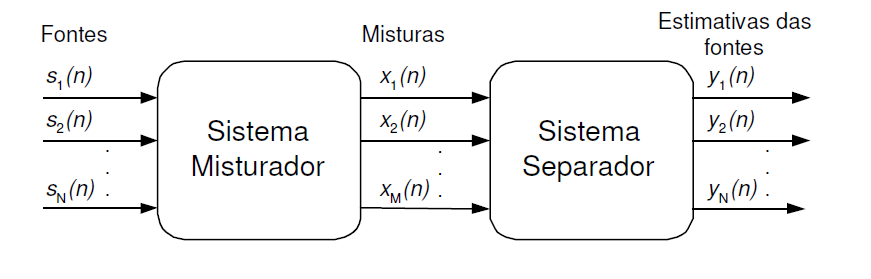
\includegraphics[scale=0.6]{model.PNG}\hspace*{\fill}
        \caption{Estrutura do problema de Separação Cega de Fontes.}
        \label{fig:structure}
    \end{figure}


\section{Aplicabilidade}
    Devido à generalidade do problema de BSS, várias aplicações podem se beneficiar dos métodos desenvolvidos para encontrar as melhores soluções. Veremos, nesta seção, algumas aplicações de destaque das técnicas de BSS nas diferentes áreas.
    
\subsection{Biomedicina}
    Na biomedicina, a busca por métodos não-invasivos que sejam confiáveis é um desafio. O EEG (Eletroencefalograma) e o ECG (Eletrocardiograma) são dois exemplos bem comuns de técnicas que satisfazem esta necessidade. Entretanto, é relativamente difícil captar apenas os sinais desejados quando os sensores são posicionados em uma determinada região do corpo humano, principalmente devido à interferência proveniente de sinais gerados por outras atividades fisiológicas.
       
    Uma forma de resolver este problema está na repetição da realização do exame, o que pode não ser viável em certas ocasiões, além de causar fadiga nos pacientes. O emprego de técnicas de BSS oferece uma alternativa eficiente, uma vez que o processamento é dado após a coleta dos dados e requer apenas um experimento.
    
    Existe uma expressiva gama de trabalhos acerca de separação de sinais biomédicos, o que evidencia sua importância.
    
\subsection{Telecomunicações}

    A BSS está diretamente ligada a um tema relevante em telecomunicações: a equalização de canais. A idéia essencial de um sistema de comunicação é fazer com que a informação enviada por um transmissor possa ser obtida de maneira tão fiel ao original quanto possível por um receptor. Assim sendo, mitigar distorções introduzidas pelo canal é fundamental. Em outra estratégia, a equalização do canal, utiliza-se um filtro (equalizador) no receptor de modo que este seja capaz de reduzir significativamente os efeitos do canal. Em essência, o desenvolvimento de técnicas de equalização está intimamente relacionado à concepção de critérios que guiem o ajuste dos parâmetros livres do equalizador de modo que se obtenha uma boa estimativa do sinal transmitido.
    Por exemplo, em um dos paradigmas mais conhecidos, adota-se como critério a minimização do erro quadrático médio entre a saída do equalizador e o sinal desejado, no caso, o sinal transmitido \cite{Haykin}. Os critérios presentes na equalização não-supervisionada (ou cega) utilizam, além dos sinais recebidos, apenas algumas informações estatísticas dos sinais transmitidos. Uma vantagem desta estratégia em relação ao paradigma supervisionado é a possibilidade de realizar o ajuste dos parâmetros concomitantemente com a transmissão dos dados.
    
\subsection{Separação de sinais de áudio}

    Imagine a seguinte situação: uma pessoa se encontra em uma sala onde existem diversos grupos de pessoas conversando concomitantemente, como, por exemplo, em uma reunião. Além disso, há ruído de fundo gerado, por exemplo, por música ambiente e ecos no recinto. Apesar de todas essas interferências, o ser humano é capaz de distinguir a voz ou o som de interesse em um determinado momento. Essa habilidade é conhecida na literatura como \textit{cocktail-party effect} \cite{cocktail}, justamente pela analogia com o cenário descrito.

    Este caso levou ao questionamento: será possível a um sistema de processamento artificial alimentado apenas por gravações de microfones posicionados pela sala distinguir o sinal de voz de uma pessoa qualquer? Ao passo que o cérebro humano resolve com certa facilidade este problema, o desenvolvimento de sistemas automáticos para realizar tal tarefa ainda corresponde a um complexo desafio.

\section{Modelagem Matemática do Problema}\label{sec:model}
    Neste capítulo, iremos descrever como o problema de BSS pode ser resolvido. Primeiramente, é necessário buscar modelos matemáticos capazes de expressar o comportamento do sistema em função do misturador e do separador.
    
    Considere que cada elemento do vetor $\mathbf{s}$($\mathpzc{n}$) = [${s_1}$($\mathpzc{n}$) ${s_2}$($\mathpzc{n}$) \dots  $s_N$($\mathpzc{n}$)]$^T$ corresponde a um sinal da fonte emissora. Analogamente, representamos os sinais misturados pelo vetor  $\mathbf{x}$($\mathpzc{n}$) = [${x_1}$($\mathpzc{n}$) ${x_2}$($\mathpzc{n}$) \dots  ${x_M}$($\mathpzc{n}$)]$^T$. De forma generalizada, o sistema misturador pode ser representado pela expressão:

    \begin{equation}\label{eq:mixer}
        \mathbf{x}(\mathpzc{n}) = \mathcal{F}(\mathbf{s}(\mathpzc{n}), \mathbf{s}(\mathpzc{n-1}), \dots, \mathbf{s}(\mathpzc{n - L}), \mathbf{v}(\mathpzc{n}))
    \end{equation}
    onde o operador $\mathcal{F}$($\cdot$) descreve a ação do sistema misturador, $L$ corresponde ao número de amostras passadas (memória) do vetor de fontes e o vetor $\mathbf{v}$($\mathpzc{n}$) corresponde ao ruído associado às fontes ou sensores do sistema.
    
    Vale ressaltar que a representação (\ref{eq:mixer}) tem caráter puramente didático, uma vez que não existem técnicas de BSS que lidem com todos estes efeitos representados e uma só vez. Em geral, as técnicas são aplicadas a casos específicos, isto é, versões simplificadas da formulação citada. Desta forma, torna-se necessário introduzir os conceitos de classificação de um sistema misturador para auxiliar na adequação do problema para o caso proposto por este trabalho.
    
    \textbf{Sistemas Lineares e Não-Lineares} Para fins de simplificação, considera-se uma mistura linear ($L=0$) e que não haja ruídos no ambiente ($\mathbf{v}(n)=0$). O sistema misturador é dito linear se o operador  $\mathcal{F}(\cdot)$ respeita o princípio da superposição, conforme descrito abaixo:
        % Linearidade
        \begin{equation}\label{eq:linearity}
            \mathcal{F}(\mathpzc{a_1}\mathbf{s_1}(\mathpzc{n}) + \mathpzc{a_2}\mathbf{s_2}(\mathpzc{n})) = \mathpzc{a_1}\mathcal{F}(\mathbf{s_1}(\mathpzc{n})) + \mathpzc{a_2}\mathcal{F}(\mathbf{s_2}(\mathpzc{n}))
        \end{equation}
    para quaisquer constantes $\mathpzc{a_1}$ e $\mathpzc{a_2}$ e vetores $\mathbf{s_1}$ e $\mathbf{s_2}$. Caso contrário, o sistema é classificado como não-linear. 
    
     \textbf{Sistemas Instântaneos e Convolutivos} Nos casos em que o sistema depende de amostras passadas, isto é, $L>0$, o sistema é dito convolutivo. No caso em que $L=0$, o sistema é dito instantâneo.
    
     \textbf{Sistemas Sub-Determinados, Determinados e Sobre-Determinados} Quando o número de sensores é maior que o número de fontes ($M>N$), tem-se o caso sobre-determinado. Analogamente, o caso sub-determinado corresponde ao caso em que $M<N$. O caso em que $M=N$ é chamado de determinado.
     
     Apesar de a característica principal da BSS ser a falta de informação sobre o processo de mistura, é fundamental ao menos ter-se um certo conhecimento sobre a estrutura do sistema misturador. Assim, é possível definir um separador estruturalmente capaz de reverter a ação do processo de mistura. Geralmente, este tipo de informação é obtido com base na aplicação de interesse. No caso deste trabalho, o problema de separação de sinais de áudio, o processo de mistura é geralmente convolutivo, devido à presença de reverberações no ambiente.
     
     A maioria dos trabalhos acerca de BSS aborda cenários com sistemas misturadores lineares e com o mesmo número de fontes e sensores, diferenciando-se basicamente no contexto de misturas instantâneas ou convolutivas. Apesar de esta última classificaçãço desempenhar um papel fundamental na abordagem do problema, o  processo de mistura pode ser igualmente descrito matematicamente da seguinte forma
     
     % Notação Matricial
     \begin{equation}\label{eq:xn}
        \mathbf{x} = \mathbf{A}\mathbf{s}
    \end{equation}
    onde a matriz $\mathbf{A}$ de dimensão ${N \times N}$ é chamada de matriz de mistura. A diferença é que, no caso instantâneo, os elementos da matriz $\mathbf{A}$ são constantes que multiplicam as componentes do vetor de fontes $\mathbf{s}$ para formar as misturas $\mathbf{x}$, enquanto no caso convolutivo, os elementos da matriz $\mathbf{A}$ são, geralmente, filtros \textit{FIR} que representam o percurso realizado pela fonte até o sensor, devido à presença de reverberação. Assim, tem-se a convolução de cada uma das respostas ao impulso desses filtros com cada elemento do vetor de fontes $\mathbf{s}$. A despeito de sua simplicidade, esta classe de modelos é válida em uma vasta quantidade de problemas de BSS \cite{ICA}. Além disso, é possível recuperar as fontes através da ICA, que será vista na próxima seção.

\section{Análise de Componentes Independentes} \label{sec:ICA}
    Nesta seção serão apresentados os aspectos básicos da ICA (do inglês \textit{Independent Component Analysis}), relacionando-a com alguns métodos semelhantes. Embora a ICA seja definida para o caso linear e convolutivo, trataremos apenas do caso linear, pois é o que condiz com a abordagem que queremos realizar, a de separação das fontes no domínio da frequência. Recomendamos ao leitor interessado em um estudo aprofundado sobre os aspectos teóricos da ICA a leitura do trabalho de Comon \cite{Comon}, responsável pela formalização matemática desse assunto, e as referências \cite{ICA3} e \cite{ICA}.
    
    Os algoritmos ICA podem ser derivados através da estimativa da máxima verossimilhança \cite{ICAML}, \cite{ML}, \cite{NaturalICA} e da maximização da não-gaussianidade \cite{fastica1}, \cite{fastica2}, \cite{fastica3} e \cite{fasticaebm}. Apesar de a maioria dos algoritmos serem desenvolvidos para trabalhar com números reais, podemos estendê-los para lidar com números complexos. Para isto, é preciso escolher apropriadamente uma função não-linear que, relacionada à formulação dos algoritmos para sinais reais, permita o emprego dos mesmos para sinais complexos.

\subsection{Definição}
    Devido à sua natureza recente, não é difícil encontrar ao menos duas definições distintas para a ICA na literatura. Entretanto, utilizaremos a definição que mais se aproxima com a aplicação que é o objetivo deste trabalho.
    
    \medskip
    
    \textbf{Definição 2.5.1 (ICA)} A ICA de um vetor aleatório $\mathbf{x}$ = [${x_1}$ ${x_2}$ $\dots$  ${x_M}]^T$ consiste em determinar o seguinte modelo generativo linear (ou modelo ICA):
    \begin{equation}\label{eq:simplifiedmixer}
        % Notação Matricial
        \mathbf{x} = \mathbf{A}\mathbf{s}
    \end{equation}
    onde os elementos de $\mathbf{s}$ = [${s_1}$ ${s_2}$ \dots  ${s_N}$]$^T$ são estatisticamente independentes entre si e $\mathbf{A}$ corresponde a uma matriz constante de dimensão $M\times N$.

    Sob a hipótese de que os sinais fontes são estatisticamente independentes entre si, fica claro que os elementos de $\mathbf{x}$ não são mais independentes, devido ao processo de mistura. O ponto fundamental da aplicação da ICA diz respeito exatamente a esta constatação, no sentido de que essa metodologia se propõe a separar as fontes a partir da recuperação da independência. O sistema separador, implementado pela matriz $\mathbf{W}$, é ajustado de modo que as compomentes do vetor $\mathbf{y}$ de estimativas das fontes sejam as mais independentes possível entre si.
    
    Entretanto, esta abordagem levanta a seguinte questão: tornar as estimativas das fontes independentes implica necessariamente na recuperação das fontes? Foi Pierre Comon \cite{Comon} que não só respondeu a esta pergunta, mas também forneceu todo o respaldo matemático necessário para o desenvolvimento da ICA e, por consequência, da BSS.
    A partir do teorema de Darmois, ele mostrou que é possível separar as fontes com base na recuperação da independência estatística, respeitando algumas condições para as fontes e para o sistema separador.

\subsection{Separabilidade}\label{sec:separability}

    O modelo descrito na Seção \ref{sec:model} é dito separável se, para toda matriz separadora $\mathbf{W}$ que resulte em um vetor $\mathbf{y}$ que tem os elementos estatísticamente independentes entre si, tem-se que $\mathbf{y}$ = $\mathbf{Wx}$ = $\mathbf{\Lambda P s}$, onde $\mathbf{\Lambda}$ e $\mathbf{P}$ representam matrizes diagonal e de permutação, respectivamente. Assim, em um modelo separável, é possível obter as fontes através da ICA. Entretanto, é importante ressaltar que surgem duas ambiguidades associadas a este modelo: a ordem das fontes e seus ganhos de escala. Mediante este problema, Comon \cite{Comon} formulou o seguinte teorema, evidenciando as condições necessárias para que um sistema misturador linear seja separável:
    
    \bigskip
    
    \textbf{Teorema 2.5.1 (Separabilidade)} Para o caso determinado ($M=N$), o modelo $\mathbf{x=As}$ é separável se e somente se a matriz $\mathbf{A}$ possuir posto completo e, no máximo, um dos elementos do vetor $\mathbf{s}$ for gaussiano.
    
    \bigskip
    
    Este teorema inclui mais uma restrição à aplicação da ICA, que é a incapacidade de recuperar fontes gaussianas. Na próxima seção, trataremos da utilização de estatísticas de segunda ordem para realizar a separação e este problema será mais bem ilustrado. Também discutiremos porque a utilização da correlação, uma medida mais ``fraca", não é capaz de resolver o problema, mas pode ser bastante útil numa etapa de pré-processamento.
  
\subsection{Técnicas baseadas em estatístiscas de segunda ordem aplicadas à BSS}\label{secondorder}

    Até a década de 1980, a maioria das técnicas de filtragem estatística eram baseadas em estatísticas de segunda ordem. Isto era devido à simplicadade matemática relacionada a este tipo de abordagem e ao fato de que modelos gaussianos de sinais eram praticamente os únicos utilizados. 
    
    Foi durante o desenvolvimento da teoria de filtragem não-supervisionada, dentro do contexto de identificação e equalização cega, que se chegou à conclusão de que, para resolver essa classe de problemas, era necessário utilizar \textit{HOS} \cite{HOS}. Em BSS, esse conhecimento é fundamental.
    
    Na seção anterior mostramos que o problema da BSS pode ser resolvido com base na independência estatística, isto é, através de \textit{HOS}, uma vez que a independência requer conhecimento da densidade de probabilidade e, por consequência, todas as estatísticas de uma variável aleatória. Entretanto, esta seção será voltada para a apresentação da abordagem utilizando apenas estatísticas de segunda ordem para BSS, mostrando que isto não é suficiente para a resolução do problema.
    
    \subsubsection{Descorrelação}
    Com base no modelo ICA apresentado na Seção \ref{sec:model}, obtemos a matriz de correlação entre as misturas, dada por:
    \begin{equation}
        \label{eq:correlationmatrixforx}
        \begin{split}
        \mathbf{R_x} & = \mathpzc{E}\{\mathbf{xx^T}\}\\
                     & = \mathpzc{E}\{\mathbf{(As)(As)^T}\}\\
                     & = \mathpzc{E}\{\mathbf{Ass^TA^T}\} \\
                     & = \mathbf{A}\mathpzc{E}\{\mathbf{ss^T}\}\mathbf{A^T} \\
                     & = \mathbf{A}\mathbf{R_s}\mathbf{A^T} \\
                     & = \mathbf{A}\mathbf{A^T}, \\
        \end{split}
    \end{equation}
    onde $\mathbf{R_s}$ corresponde à matriz de correlação do vetor das fontes. Como estamos utilizado a hipótese de que as fontes são estatísticamente independentes e possuem variância unitária, esta matriz é igual à identidade.
    
    Após passar por um sistema separador, a correlação entre as estimativas das fontes é descrita por:
    \begin{equation}
        \label{eq:correlationmatrixfory}
        \begin{split}
        \mathbf{R_y} & = \mathpzc{E}\{\mathbf{yy^T}\}\\
                     & = \mathpzc{E}\{\mathbf{(Wx)(Wx)^T}\}\\
                     & = \mathpzc{E}\{\mathbf{Wxx^TW^T}\} \\
                     & = \mathbf{W}\mathpzc{E}\{\mathbf{xx^T}\}\mathbf{W^T} \\
                     & = \mathbf{W}\mathbf{R_x}\mathbf{W^T}\\
        \end{split}
    \end{equation}
    
    Assim, para descorrelacionarmos as saídas do sistema separador, precisamos determinar $\mathbf{W}$ tal que $\mathbf{R_y = I}$. Solucionando a equação, chegamos à conclusão que
    \begin{equation}
        \label{eq:separationmatrixsolution}
        \mathbf{W} = \mathbf{D}^{-\frac{1}{2}}\mathbf{E^T}
    \end{equation}
    onde $\mathbf{E}$ e $\mathbf{D}$ representam as matrizes de autovetores e autovalores da matriz de correlação $\mathbf{R_x}$, respectivamente.
    
    Entretanto, se consideramos o caso em que o sistema separador é dado pela expressão $\mathbf{QW}$, onde $\mathbf{Q}$ corresponde a uma matriz ortogonal (i.e., sua inversa coincide com sua transposta), substituindo na solução da equação (\ref{eq:correlationmatrixfory}), é possível verificar que o resultado obtido na equação (\ref{eq:separationmatrixsolution}) permanece o mesmo. Isto mostra que a recuperação das fontes utilizando apenas a informação da descorrelação apresenta uma indeterminação relacionada a um fator ortogonal.
    
    A seguir, ilustramos geometricamente o problema. Com este objetivo, exibimos nas Figuras \ref{fig:first_sub}, \ref{fig:second_sub} e \ref{fig:third_sub} as distribuições conjuntas de duas fontes, as misturas e suas estimativas obtidas pelo processo de branqueamento, respectivamente. Como o sistema misturador linear é modelado por uma matriz, as misturas são geradas a partir de rotações e escalonamentos das fontes. Apesar do braqueamento conseguir recuperar as escalas das fontes, ele não consegue recuperar a rotação devido à indeterminação referente a uma matriz ortogonal, cujo efeito é a rotação dos dados.
    
    Esta ineficácia na recuperação de fontes gaussianas mostra a limitação da estatística de segunda ordem. Entretanto, a aplicação do branqueamento como um pré-processamento pode ajudar bastante no processo de separação, visto que este faz aproximadamente metade do trabalho de separação.
    
\begin{figure}
    \centering
    \subfigure[Distribuição conjunta das fontes.]
    {
        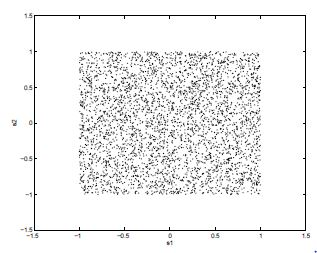
\includegraphics[scale=0.8]{distrib_fontes.JPG}
        \label{fig:first_sub}
    }
    \subfigure[Distribuição conjunta das misturas.]
    {
        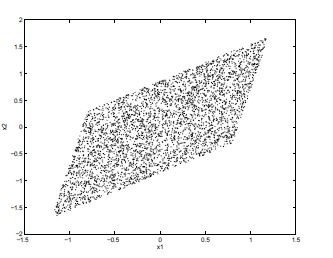
\includegraphics[scale=0.8]{distrib_misturas.JPG}
        \label{fig:second_sub}
    }
    \\
    \subfigure[Distribuição conjunta das estimativas.]
    {
        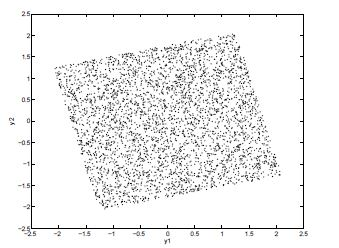
\includegraphics[scale=0.8]{distrib_estimat.JPG}
        \label{fig:third_sub}
    }
    \caption{Tratamento da BSS considerando estatística de segunda ordem. Na Figura (a), as distribuições de probabilidade de duas fontes $\mathbf{s_1}$ e $\mathbf{s_2}$ estão representadas nos eixos da abscissa e ordenada, respectivamente. Para estas duas fontes, obtemos uma distribuição conjunta que fica inteiramente contida dentro de um quadrado de lado 2. Na Figura (b), as distribuições de probabilidade de duas misturas $\mathbf{x_1}$ e $\mathbf{x_2}$ obtidas a partir das fontes $\mathbf{s_1}$ e $\mathbf{s_2}$ estão representadas nos eixos da abscissa e ordenada, respectivamente. O processo de mistura resultou em uma mudança de escala e de rotação das densidades de probabilidade das fontes originais $\mathbf{s_1}$ e $\mathbf{s_2}$. Na Figura (c), as distribuições de probabilidade dos vetores estimados $\mathbf{y_1}$ e $\mathbf{y_2}$, obtidos através da descorrelação, estão representadas nos eixos da abscissa e ordenada, respectivamente. Nota-se que apenas a escala das fontes originais foi recuperada. }
    \label{fig:sample_subfigures}
\end{figure}


\subsection{Modelo de maximização da não-gaussianidade}
    
    Um dos principais atrativos presentes nessa estratégia é a possibilidade de recuperar cada uma das fontes individualmente. Um dos algoritmos mais conhecidos em BSS, o FastICA \cite{fastica1}, se baseia neste critério. Para entendermos a abordagem via maximização da não-gaussianidade, precisamos introduzir o conceito de medição da independência entre duas estimativas de fontes, observando sua não-gaussianidade. Para isso, utiliza-se o Teorema Central do Limite \cite{cetrallimit}, que diz que dadas $n$ variáveis aleatórias independentes $\mathpzc{x_i}$, se formamos sua soma $\mathpzc{x = x_1 + \dots + x_n}$, sendo esta uma variável aleatória com média $\mathpzc{\eta = \eta_1 + \dots + \eta_n}$ e variância $\mathpzc{\sigma^2 = \sigma_1^2 + \dots + \sigma_n^2}$, dentro de certas condições gerais, a distribuição ${F(x)}$ de $\mathpzc{x}$  se aproxima de uma distribuição normal com a mesma média e variância à medida que ${n}$ cresce.
    
    \medskip
    
    Em termos práticos, quanto mais fontes compuserem uma mistura, mais gaussiana ela será. Existem duas formas de medir a gaussianidade: a curtose e a negentropia.

\subsubsection{Curtose}
    
    A curtose é uma estatística de quarta ordem que categoriza as distribuições como gaussiana, subgaussiana e super-gaussiana. Também pode ser interpretada como o grau de desvio da inclinação em relação à curva de uma distribuição gaussiana, sendo definida como
    
    \begin{equation}
        \mathpzc{k_4} = \mathpzc{E}\{\mathpzc{x^4}\} - 3(\mathpzc{E}\{\mathpzc{x^2}\})^2.
    \end{equation} 
    
    A curtose é não-nula para a grande maioria das variáveis aleatórias, salvo os sinais gaussianos. Assim, podemos estender o conceito de maximização da não-gaussianidade para a maximização do valor absoluto da curtose do conjunto das fontes. Essa abordagem foi proposta em \cite{ML}, juntamente à deflação, que tem por objetivo a extração das fontes de maneira sequencial.
    
    Segundo o autor em \cite{LuizVictorio}, a derivação do algoritmo de maximização da curtose resulta em:
    \begin{equation}
        \mathbf{w_i} \leftarrow \mathbf{w_i} + \eta  sign(curt_{ICA}(\mathbf{w_iz}))\mathpzac{E}\{\mathbf{z^T}(\mathbf{w_iz})^3\}
        \label{eq:refreshforcurtosis}
    \end{equation}
    \begin{equation}
        \mathbf{w_i} \leftarrow \frac{\mathbf{w_i}}{|| \mathbf{w_i}||},
    \end{equation}
    onde o termo $curt_{ICA}$ tem a seguinte definição:
    \begin{equation}
        curt_{ICA} = \mathpzc{E}\{(\mathpzc(y - \mu_y)^4\} -3\sigma_y^4
    \end{equation}

    Existem basicamente duas abordagens para este caso: a baseada em um gradiente (que faz com que o mesmo necessite de uma escolha eficiente para passo de adaptação, podendo resultar em convergência lenta ou até mesmo divergência) e a de ponto fixo, que é a base do FastICA \cite{fastica1}. 
    
    Sobre a abordagem de ponto fixo, seja $\mathpzc{f}$ uma função definida para todos os números reais. A partir de um ponto inicial $\mathpzc{x_0}$, a regra de iteração para o ponto fixo se dá através de 
    \begin{equation}
        \mathpzc{x_{n+1}} = \mathpzc{f(x_n)}, \mathpzc{n = 0,1,2,}\dots,
    \end{equation}
    gerando uma sequência que converge para um ponto fixo da função dado por
    \begin{equation}
        \mathpzc{f(x_{FP})} = \mathpzc{x_{FP}}.
    \end{equation}
    Para que este algoritmo convirja para este ponto estável, o gradiente deve apontar na direção de $\mathbf{w_i}$. Somente assim, quando adicionarmos o gradiente a $\mathbf{w_i}$ em (\ref{eq:refreshforcurtosis}), o vetor $\mathbf{w_i}$ manterá a sua direção, apesar de sua norma $\mathbf{||w_i||}$ se modificar. A abordagem do FastICA propõe algumas simplificações \cite{fastica1}, chegando ao algoritmo na sua forma final:
    
    \begin{equation}
        \mathbf{w_i} \leftarrow \mathpzac{E}\{\mathbf{z^T}(\mathbf{w_iz})^3\} - 3\mathbf{w_i}
        \label{eq:ICAcurtosis}
    \end{equation}
     \begin{equation}
        \mathbf{w_i} \leftarrow \frac{\mathbf{w_i}}{||\mathbf{w_i}||}
        \label{eq:ICAcurtosismodulate}
    \end{equation}

    \bigskip

    Entretanto, o problema com \textit{outliers}, que correspondem às observações da amostra que desviam completamente das demais, tem bastante influência na pouca utilização do método, uma vez que um \textit{outlier} pode mudar completamente a curtose. Por conta disto, neste trabalho não serão abordados algoritmos que utilizem este conceito.
    
\subsubsection{Negentropia} \label{sec:negentropy}

    Já a abordagem da negentropia é mais robusta, apesar de ser computacionalmente mais intensa. Entretanto, existem aproximações simples que garantem um resultado satisfatório nesta abordagem. A entropia é um conceito da Teoria da Informação e está relacionada à incerteza associada a uma variável aleatória. Quanto maior o seu valor, mais aleatória é a variável. Um resultado fundamental da Teoria da Informação é de que uma variável contínua com distribuição gaussiana tem a maior entropia diferencial entre todas as variáveis de igual variância \cite{entropy}. Assim, uma forma de maximizar a não-gaussianidade seria minimizar as entropias marginais das estimativas das fontes. Um problema da entropia diferencial é que seu valor é alterado quando a variável aleatória é multiplicada por uma constante. Para resolver este problema, introduzimos o conceito de negentropia, que é uma normalização da entropia de forma que fique invariante a qualquer transformação linear invertível. A negentropia de uma variável aleatória $\mathpzc{x}$ é dada por:
    \begin{equation}
        \mathpzc{J(x) = H(x_g) - H(x)},
    \end{equation}
    onde $\mathpzc{x_g}$ representa uma variável aleatória gaussiana com a mesma variância de $\mathpzc{x}$. Desta forma, a negentropia é sempre não-negativa e só é igual à zero quando $\mathpzc{x}$ for uma variável gaussiana. Uma vantagem da negentropia é que esta medida de gaussianidade é consideravelmente mais robusta a \textit{outliers} se comparada à curtose.
    Entretanto, há uma dificuldade em relação à sua aplicação devido à necessidade de estimação da entropia. Para tentar contornar isto, é comum escolher uma função não-linear não-quadrática $G(\cdot)$ e incorporá-la à formulação tradicional do método \cite{fastica1}, dada por:
    \begin{equation}
        \mathpzc{J(y)} = \alpha(\mathpzc{E}\{\mathpzc{G(y)}\} - \mathpzc{E}\{\mathpzc{G(\nu)}\})^2,
    \end{equation}
    onde $\alpha$ é uma constante e $\nu$ é uma variável aleatória gaussiana de média zero e variância unitária.  O algoritmo de adaptação da matriz separadora usando maximização da negentropia é dado por:
    \begin{equation}
          \mathbf{w_i} \leftarrow  \mathbf{w_i} + \eta[\mathpzc{E}\{\mathpzc{G(\nu)}\} - \mathpzc{E}\{\mathpzc{G}\mathbf{w_iz}\}]\mathpzc{E}\{\mathbf{z^Tg(w_iz)}\}
    \end{equation}
    \begin{equation}
          \mathbf{w_i} \leftarrow  \frac{\mathbf{w_i}}{||\mathbf{w_i}||},
    \end{equation}
    onde $\mathpzc{g} = \mathpzc{G}'$ é a primeira derivada da função não-quadratíca $\mathpzc{G}$.
    Assim como o caso da curtose, também é possível derivar o algoritmo de ponto fixo para este caso. Conforme descrito em \cite{LuizVictorio}, encontra-se o seguinte algoritmo:
    
    \begin{equation}
        \mathbf{W} \leftarrow \mathpzc{E}\{\mathpzc{g}\mathbf{(y)z^T}\} - diag(\mathpzc{E}\{\mathpzc{g'}\mathbf{(y)}\}\mathbf{W}
    \end{equation}
    
    \begin{equation}
        \mathbf{W} \leftarrow (\mathbf{WW^T})^{-\frac{1}{2}}\mathbf{W}
    \end{equation}
    
    
    Assim sendo, resta escolhar uma função \textit{G} que contenha boas propriedades de convergência ao mesmo tempo que seja uma boa aproximação da entropia. A função $G(s_i)$ = -log($q(s_i)$), onde $q(s_i)$ é a densidade de probabilidade estimada da fonte $s_i$ é uma escolha natural. O problema se torna estimar as densidades de probabilidade das fontes, mas na Figura \ref{fig:scoretable} exibimos as densidades de probabilidade em conjunto com as chamadas funções $g$, também chamadas de funções \textit{score}.
    
    \begin{figure}
        \centering
        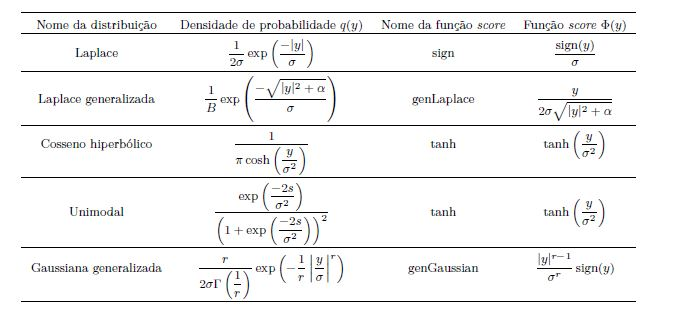
\includegraphics[scale=0.7]{table.JPG}
        \caption{Funções score para diferentes densidades de probabilidade de fontes reais.}
        \label{fig:scoretable}
    \end{figure}
    
\subsection{Modelo de estimação por máxima verossimilhança}

    A maioria dos critérios utilizados pelo caso linear da BSS, embora tenha ligações com o ICA, surgiu a partir de outras idéias que não necessariamente estão ligadas à independência estatística. O caso da estimação por máxima verossimilhança é um dos exemplos mais consagrados deste grupo. Apresentaremos, nesta seção, seus conceitos e como a mesma se relaciona com o problema de BSS. 
    O objetivo por trás da ML (do inglês \textit{Maximum Likelihood}) é determinar um conjunto de parâmetros $\mathbf{\theta} = [\theta_1, \dots, \theta_n]$ a partir de um conjunto de amostras $\mathbf{e} = [e(1), \dots, e(P)]$ que contém informações sobre eles. As estimativas de $\mathbf{\theta}$ são denotadas por $\hat{\theta}$ e determinadas através da maximização da chamada função de máxima verossimilhança $\mathbf{L(\theta)}$, conforme    
    \begin{equation}\label{eq:argmax}
    \hat{\theta} = \operatorname*{arg\,max}_{\theta} \mathbf{L(\theta)}
    = \operatorname*{arg\,max}_{\theta}
    \mathpzc{p_e}(\mathbf{e} | \mathbf{\theta})
    \end{equation} ou seja, a abordagem por máxima verossimilhança busca o conjunto de parâmetros que maximiza a probabilidade condicional de $\mathbf{e}$ dado $\mathbf{\theta}$.
    
    É comum assumir a independência estatística entre as amostras de $\mathbf{e}$. Assim sendo, podemos reescrever a função de máxima verossimilhança como
    
    \begin{equation}\label{eq:argmax2}
        \mathbf{L(\theta)}
        =\mathpzc{p_e}(\mathbf{e} | \mathbf{\theta})
        =\prod_{p=1}^P \mathpzc{p_e}(\mathbf{e}(\mathpzc{p}) | \mathbf{\theta})
    \end{equation}

    Com relação ao emprego da estimação por máxima verossimilhança no problema de BSS, os parâmetros a serem determinados são os elementos da matriz de mistura $\mathbf{A}$ e os dados disponíveis são as amostras do vetor de misturas $\mathbf{x}$. Assim, segundo \cite{cetrallimit} e considerando a hipótese de independência entre as fontes, temos:
        \begin{equation}\label{eq:verobss}
          \begin{split}
         \mathbf{L(A)} & =\prod_{p=1}^P \mathpzc{p_x}(\mathbf{x}(\mathpzc{p}) | \mathbf{A})\\
                                & =\prod_{p=1}^P\frac{\prod_{n=1}^N\mathpzc{p_{s_n}}(\mathbf{\tilde{a_n}}\mathbf{x}(\mathpzc{p}))}{| det(\mathbf{A}) |},
        \end{split}
    \end{equation} 
    onde o termo $\mathbf{\tilde{a}_n}$ corresponde a $\mathpzc{n}$-ésima linha da matriz inversa de $\mathbf{A}$. Também é possível descrever a função de máxima verossimilhança em termos da matriz separadora $\mathbf{W}$, dada por:
    \begin{equation}
        \label{eq:veroForW}
        \mathbf{L(W)} = \prod_{p=1}^{P}\prod_{i=1}^N\mathpzc{p_{s_n}}(\mathbf{w_nx}(\mathpzc{p}))|\text{det}(\mathbf{W})|
    \end{equation}
  
    Entretanto, é comum utilizar-se do logaritmo da verossimilhança, uma vez que é algebricamente mais simples e o máximo ainda é encontrado no mesmo ponto. Assim sendo, obtemos a equação
    
        \begin{equation}
        \label{eq:logverossimilance}
        log(\mathbf{L(W)}) = \mathpzc{E}\{\sum_{i=1}^Nlog(\mathpzc{p_{s_n}}(\mathbf{w_nx}(\mathpzc{p})) + \text{P log}(|det(\mathbf{W})|)\}
    \end{equation}
    onde o operador $\mathpzc{E}\{\cdot\}$ representa a estimativa do valor esperado. O valor máximo da verossimilhança pode ser encontrado iterativamente, utilizando-se o gradiente estocástico da verossimilhança. Dois dos principais algoritmos que utilizam a estimativa ML são o Natural ICA \cite{NaturalICA} e o algoritmo Bell-Sejnowski \cite{ICAML}.
    
    O algoritmo Bell-Sejnowski converge muito lentamente, devido à inversão da matriz separadora $\mathbf{W}$. Este é um caso onde o processo de branqueamento, apresentado na Seção \ref{sec:separability}, e que será visto novamente à frente, ajuda bastante na convergência. Entretanto, o Natural ICA possui uma convergência melhor sem precisar necessariamente de um pré-processamento, tornando o algoritmo Bell-Sejnowski obsoleto.
    
    O gradiente, segundo a definição matemática tradicional, aponta para a direção de maior crescimento em um espaço Euclidiano. Porém, o espaço de busca de parâmetros no ICA não é sempre Euclidiano, mas tem uma estrutura métrica Riemaniana \cite{Riemenn}. Neste caso, deve ser utilizado o chamado gradiente natural, que aplicado à verossimilhança em (\ref{eq:veroForW}), dá origem ao algoritmo Natural ICA.
    
    Definindo-se por $\mathcal{J}$ a função objetivo em função do parâmetro $\mathbf{W}$, temos que o gradiente usual e o gradiente natural são dados, respectivamente, por
    
    \begin{equation}
        \label{eq:gradiente}
        \nabla\mathpzc{J} = \frac{\partial \mathpzc{J}(\mathbf{W})}{\partial \mathbf{W}}
    \end{equation}
    \begin{equation}
        \label{eq:naturalgradiente}
        \nabla\mathpzc{J} = \frac{\partial \mathpzc{J}(\mathbf{W})}{\partial \mathbf{W}}\mathbf{W^T}\mathbf{W}
    \end{equation}
    onde a diferença reside na inclusão do produto com o termo quadrático de $\mathbf{W}$ para o caso do Natural ICA.
    
    A atualização da matriz separadora $\mathbf{W}$ é dada em (\ref{eq:refresh}). Esta equação depende apenas das amostras $\mathbf{y}$ e não possui nenhuma restrição. Isto torna essa abordagem bastante vantajosa, pois mesmo que a matriz misturadora $\mathbf{A}$ seja mal condicionada, o desempenho é bastante satisfatório. A demonstração matemática desta equação encontra-se em \cite{ICA3}.
    
    \begin{equation}
    \label{eq:refresh}
    \mathbf{W} \leftarrow \mathbf{W} + \eta(I - \mathpzc{E}\{\phi({\mathbf{y})\mathbf{y^T}}\})\mathbf{W}
    \end{equation}
    
    A função $\phi$ é chamada de \textit{score} e é calculada baseada na densidade de probabilidade das fontes através da equação
    
    \begin{equation}
    \label{eq:score}
    \mathbf{\phi({\mathpzc{y_i}})} = - \frac{\partial}{\partial \mathpzc{y_i}} \log(p_y(\mathpzc{y_i})).
    \end{equation}
    
    As densidades de probabilidade das fontes devem ser estimadas, e devem ser não-gaussianas. Apesar de não precisarem ser exatas, há um limite para o quão erradas estas estimativas podem estar. Uma análise quantitativa deste erro é dada em \cite{ICA3}, considerando o algoritmo Bell-Sejnowski e passos de adaptação pequenos.
    
    Vale ressaltar que supor que a distribuição das fontes é conhecida é uma desvantagem dos algoritmos baseados em ML em relação aos algoritmos que utilizam maximização da não-gaussianidade. No caso em que a distribuição estimada é bem diferente da distribuição real, os algoritmos baseados em ML terão desempenho inferior aos algoritmos baseados em maximização da não-gaussianidade, mesmo sem a restrição de que a matriz separadora seja unitária. A Figura \ref{fig:scoretable} relaciona algumas das densidades de probabilidade para fontes reais utilizadas no algoritmo Natural ICA e suas respectivas funções score.
    
    Existem particularidades de certos casos que geram a necessidade de certas modificações no algoritmo. No caso do Natural ICA, para fontes cujas potências variam muito de um instante do tempo para o outro, o algoritmo pode ter problemas para convergir, devido à sua relação com o gradiente. Isto acontece em uma implementação on-line, por exemplo. Para este caso, em \cite{holonomic} é derivado o Natural ICA com restrições não-holonômicas. Entretanto, por não fazer parte do escopo deste trabalho, esta abordagem não será discutida.


\section{Avaliação de Desempenho}
    Utilizamos a avaliação de desempenho proposta por \cite{performance}, sendo:
    
    \begin{equation}
         y_i(n) = [s_{target}]_i(\mathpzc{n})  + [e_{art}]_i(\mathpzc{n})  +  [e_{noise}]_i(\mathpzc{n}) +  [e_{interf}]_i(\mathpzc{n})
    \end{equation}
    e as métricas propostas:
    
    \begin{enumerate}
        \item SIR (Razão Sinal-Interferência) - mede a razão entre as potências do sinal da fonte desejada e da interferência de outras fontes;
        \item SDR (Razão Sinal-Distorção) - mede a razão entre as potências do sinal desejado e das distorções provenientes de ruído, janelamento, transformações não-lineares, e de outras fontes;
        \item SAR (Razão Sinal-Artefatos) - mede a razão entre as potências do sinal de saída (com interferências e ruído) e dos artefatos, que são todas as distorções do sinal excluídas as interferências de outras fontes e o ruído dos sensores.
    \end{enumerate}
    
    Estas medidas podem ser expressas pelas seguinte forma:
    
    \begin{equation}
        \label{eq:sir}
        SIR_i = 10\log_{10} \frac{|| [s_{target}]_i ||^2}{|| [e_{interf}]_i ||^2},
    \end{equation}
    \medskip
    \begin{equation}
        \label{eq:sdr}
        SDR_i = 10\log_{10} \frac{|| [s_{target}]_i ||^2}{|| [e_{interf}]_i + [e_{noise}]_i + [e_{art}]_i   ||^2},
    \end{equation}
    \medskip
    \begin{equation}
        \label{eq:sar}
        SAR_i = 10\log_{10} \frac{|| [s_{target}]_i + [e_{interf}]_i + [e_{noise}]_i ||^2}{|| [e_{interf}]_i ||^2},
    \end{equation}
    onde $s_{target}$ é a fonte real, com alguma distorção aceitável, $e_{interf}$  é a parcela do erro
proveniente de interferências de outras fontes $i`$ $\neq$ i na estimativa $y_i$ da fonte, $e_{noise}$
é a parcela do erro proveniente de ruído dos sensores, e $e_{art}$ é a parcela do erro que não provém nem de interferências nem de ruído. Estes podem ser obtidos pelas seguintes equações:

    \begin{equation}
        \label{eq:star}
         [s_{target}]_i  = (\mathbf{y_i^Ts_i})\frac{\mathbf{s_i}}{||\mathbf{s_i}||^2}
    \end{equation}
    
    \medskip
    
    \begin{equation}
        \label{eq:eint}
         [e_{interf}]_i  = \sum_{i' \neq i} \{(\mathbf{y_i^Ts_i})\frac{\mathbf{s_i}}{||\mathbf{s_i}||^2}\}
    \end{equation}
    
    \medskip
    
    \begin{equation}
        \label{eq:enoise}
         [e_{noise}]_i  = (\mathbf{y_i^Tn_j})\frac{\mathbf{n_j}}{||\mathbf{n_j}||^2}
    \end{equation}
    
    \medskip
    
        \begin{equation}
        \label{eq:eart}
         [e_{art}]_i  = y_i -  [e_{noise}]_i -  [e_{interf}]_i - [s_{target}]_i 
    \end{equation}
    
    Como não consideramos ruído nos sensores neste trabalho, temos $e_{noise}$ = 0.
    
    

% ---------------------------------------------------------------
% Chapter 3 - Separação de Fontes no Domínio da Frequência
% ---------------------------------------------------------------
\chapter{Separação de Fontes no Domínio da Frequência}
\label{cap3}
\label{chap:3}

\section{Relação Tempo-Frequência}
    
    \subsection{Contexto}
        Para o caso real, os sinais de áudio são convoluídos com a resposta ao impulso de um filtro, que representa o caminho percorrido pelos mesmos das fontes aos sensores. Isto caracteriza um caso de misturas convolutivas (conforme visto na Seção \ref{sec:separability}). 
        
        Com o conhecimento de que podemos implementar a operação de convolução de sinais no domínio tempo pela  multiplicação no domínio da frequência, uma forma de simplificar este problema é aplicar a transformada de Fourier a estes sinais, resolver a separação de misturas instântaneas e aplicar a transformada inversa de Fourier para levar os sinais de volta ao domínio do tempo. Uma das vantagens desta abordagem reside na redução da complexidade computacional, estando qualquer algoritmo ICA que trabalhe com números complexos e misturas instantâneas apto para ser usado.
        
        Entretanto, as ambiguidades de escalamento e permutação inerentes ao problema de BSS (Seção \ref{sec:separability}) tornam-se elementos centrais no processo de separação e precisam ser resolvidas. Ao trabalhar no domínio da frequência, a ICA fornece componentes independentes em cada raia de frequência, mas as componentes de cada fonte devem ser corretamente agrupadas antes de serem levadas para o domínio do tempo. Isto é crucial para obter uma solução aceitável.
        
        Também é relevante citar o problema da circularidade da DFT. No caso mais geral de sinais e sistemas discretos, o produto no domínio da frequência corresponde à convolução circular no domínio do tempo. Isto restringe o uso dessa propriedade ao caso em que os filtros no domínio do tempo são periódicos, o que não é condizente com a realidade. Para fazer com que na nossa aplicação a multiplicação no domínio da frequência seja equivalente à convolução linear no domínio do tempo, é necessário que o número de raias de frequência (tamanho da DFT) seja maior ou igual ao comprimento da resposta ao impulso do filtro somado ao tamanho do trecho do sinal que está sendo processado, além do sinal ter de ser reconstruído através da técnica de \textit{Overlap-Add} \cite{signalprocessing} . Este processo é conhecido como \textit{FFT Filtering} e é amplamente utilizada para realizar a convolução rápida de um filtro de ordem elevada com um sinal longo. Quando esta condição no tamanho da DFT não é respeitada, o sinal proveniente do tratamento no domínio da frequência, seguido da sua IDFT será uma versão distorcida do sinal equivalente à convolução no domínio do tempo.
        
        Outro ponto fundamental sobre trabalhar no domínio da frequência é que introduzimos um caráter complexo aos sinais do nosso sistema devido às transformadas necessárias para a mudança de domínio. Conforme citado na Seção \ref{sec:ICA}, embora vários algoritmos ICA tenham sido desenvolvidos para trabalhar com sinais reais, eles podem ser estendidos para o caso complexo, desde que tenha sido apropriadamente escolhida a função $G$ (maximização da não-gaussianidade) ou a função \textit{score} (estimação da ML). 
        
    \subsection{Sumário}
        O processo de tratamento do problema de FDBSS, ilustrado na Figura \ref{fig:frequencymodel}, pode ser estruturado da seguinte forma:
        
        \begin{enumerate}
            \item Inicialmente, transformam-se os sinais de misturas $\mathpzc{x_j}(n)$, $j = 1,\dots,M$ em suas representações no domínio da frequência $\mathpzc{x_j}(m,k)$, $k = 0, \dots, K-1$ (sendo $m$ o índice do \textit{frame} e $K$ o número de raias de frequência), através da \textit{STFT} (do inglês \textit{Short Time Fourier Transform});
            
            \item Como etapa de pré-processamento, realiza-se o branqueamento dos sinais, obtendo-se os sinais $\mathpzc{z_j}(m,k)$ e a matriz branqueadora $\mathbf{V}$($\mathpzc{k}$);
            
            \item A etapa de processamento, que consiste na separação propriamente dita, é realizada gerando uma matriz separadora $\mathbf{W}$($\mathpzc{k}$) para cada raia de frequência $k$, além dos vetores com as saídas separadas $\mathbf{y}$($\mathpzc{m,k})$ = [$\mathpzc{y_1}$($\mathpzc{m,k})$, $\dots$, $\mathpzc{y_N}$($\mathpzc{m,k})$]$^T$;
            
            \item Como pós-processamento, são resolvidas as questões de permutação e escalamento, através das matrizes $\mathbf{P}$($\mathpzc{k})$ e $\mathbf{\Lambda}$($\mathpzc{k})$;
            
            \item Por fim, é necessário levar o vetor com as saídas separadas para o domínio do tempo através da \textit{ISTFT} (do inglês \textit{Inverse Short Time Fourier Transform}).
            
        \end{enumerate}

        \begin{figure}[h!]
            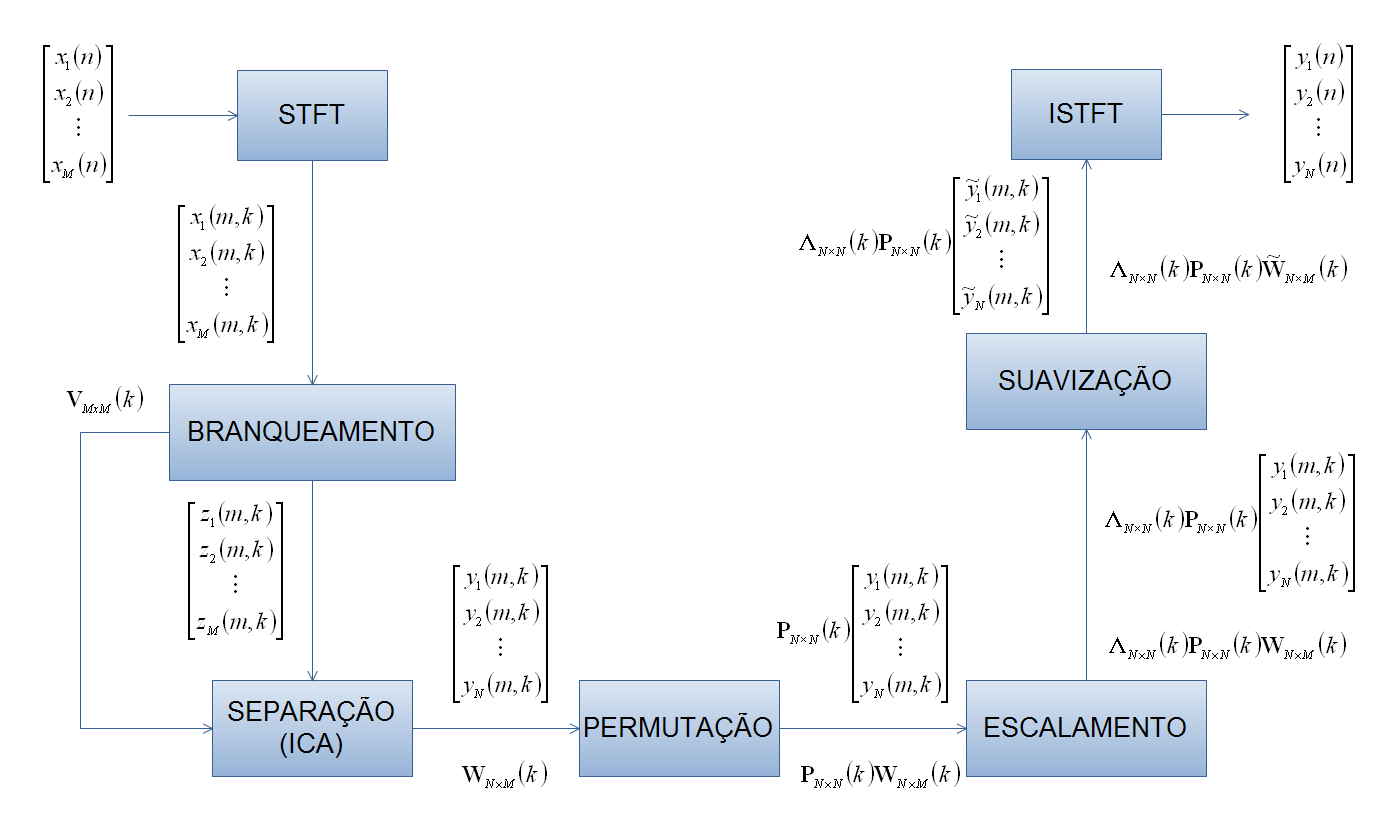
\includegraphics[scale=0.4]{frequencyprocess.png}
            \caption{Esquema do processo de FDBSS.}
            \label{fig:frequencymodel}
        \end{figure}

    \subsection{STFT} \label{sec:stft}
        A STFT de um sinal x é dada pela equação:

    %STFT
    \begin{equation}\label{eq:STFT}
        X(\mathpzc{m},\mathpzc{k})
        = \sum_{n} x(\mathpzc{n})
        \mathpzc{win}_\mathpzc{a}(\mathpzc{n} - \mathpzc{mJ})
        exp \left( -j \frac{2\pi\mathpzc{kn}}{K} \right), \mathpzc{k} = 0, \dots, K-1
    \end{equation}
    onde:
    \begin{itemize}
        
        \item $k$ é a raia de frequência, com intervalo $[0, K-1]$. Pode ser interpretada como a frequência discreta $\mathpzc{f_k}$ $\in$ \big\{0,$\frac{1}{K}$ $\mathpzc{f_s}$, \dots, $\frac{K-1}{K}$ $\mathpzc{f_s}$ \big\};
                    
        \item $K$ é o número de raias de frequência da DFT;
                    
        \item $L$ é o comprimento da janela;
                    
        \item $J$ é o deslocamento da janela;
        
        \item  $\mathpzc{f_s}$ é a frequência de amostragem;
        
        \item $\mathpzc{win_a}$($\mathpzc{n}$) é a janela de análise, definida como sendo não-nula apenas no intervalo $[0, L-1]$. O salto $J$ é obviamente menor ou igual a $L$, ou haverá perda de observações. Este salto deve ser bem escolhido para não haver distorções na síntese dos sinais.
    \end{itemize}
    
        Em geral, utiliza-se $K=L$ na equação acima. Entretanto, há casos em que $K>L$, chamados de \textit{oversampled}. Nestes casos, é necessário utilizar \textit{zero-padding} para preencher o sinal com zeros antes de passar para a frequência, conforme descrito em \cite{STFT}.
        
        Uma notação prática para o cálculo da STFT é dada por:


        \begin{equation}\label{eq:practiceSTFT}
            \mathbf{X}(\mathpzc{m})
            = DFT(diag(\mathbf{x_{frame}}(\mathpzc{m})\mathbf{win_a}))
         \end{equation}
         onde 
        \begin{enumerate}
        
            \item \textit{DFT}($\mathbf{v})$ representa a DFT do vetor $\mathbf{v}$, que pode ser eficientemente calculada através da FFT;
            
            \item O vetor $\mathbf{x_{frame}}$(m) = [$\mathpzc{x}$($\mathpzc{mJ}$), $\dots$, $\mathpzc{x(mJ + L - 1)}$]$^T$ tem comprimento $L$ e representa o \textit{frame m} no domínio do tempo;
            
            \item O vetor $\mathbf{X}(\mathpzc{m})$ = [${X}$($\mathpzc{f_0,m})$, $\dots$, ${X}$(${f_{K-1},m}$)]$^T$ tem comprimento $K$ e corresponde à representação em
            frequência do \texit{frame m};
            
            \item O vetor $\mathbf{win_a}$ contém os elementos não nulos da janela mostrada na equação (\ref{eq:STFT}). Assim sendo, tem comprimento $L$. O produto diag($\mathbf{x}$($\mathpzc{mJ}$))$\mathbf{win_a}$ resulta em um vetor de comprimento $L$. Por conta disso, se $K>L$, deve ser realizado \texit{zero-padding} de $K-L$ amostras no final do vetor, antes de aplicar a DFT.
        
        \end{enumerate}
        
        Uma notação prática correspondente ao cálculo da ISTFT está é dada pelas equações:
        
        \begin{equation}\label{eq:practiceISTFT}
            \mathbf{y_{frame}}(\mathpzc{m})
            = diag(\mathbf{win_s}IDFT(\mathbf{Y}(\mathpzc{m}))
         \end{equation}
        
        \begin{equation}\label{eq:practiceISTFT2}
            \mathbf{y}(\mathpzc{n})
            = \sum_{m}\text{shift}(\mathbf{y_{frame}}(\mathpzc{m}),\mathpzc{mJ},\mathbf{N_{amost}})
         \end{equation}
        
        O sinal $\mathbf{y}$($\mathpzc{n}$) tem o comprimento de $N_{amost}$ e a operação shift($\mathbf{a}$,b,c) desloca o vetor $\mathbf{a}$ de b amostras e aumenta seu comprimento para c, de forma que o vetor resultante tem no total $P$ elementos não-nulos, onde $P$ é o tamanho do vetor $\mathbf{a}$.
        
        A técnica de \textit{Overlap-Add} consiste em acrescentar \textit{frames} superpostos para formar o sinal completo. Também conhecida como OLA, esta técnica possui algumas variações, tais como a WOLA (\textit{Weighted Overlap-Add}) e a COLA (\textit{Constant Overlap-Add}). Esta técnica utiliza-se de uma janela de síntese $\mathpzc{win_s}(n)$ para a realização da ISTFT. Relacionar a janela de síntese $\mathpzc{win_s}(n)$ com a janela de análise $\mathpzc{win_a}(n)$ é fundamental para criar condições para que a transformação de volta para o domínio do tempo não possua distorções. 
        
        Para que a \textit{FFT Filtering} gere um resultado satisfatório, as condições (\ref{eq:condition1}) e (\ref{eq:condition2}) devem ser satisfeitas. A condição \ref{eq:condition2} é chamada de COLA.
        
        \begin{equation}\label{eq:condition1}
            K \geq L + Q - 1
        \end{equation}
        
        \begin{equation}\label{eq:condition2}
            \sum_m \mathpzc{win_a(n - mJ) = c},\text{c constante}, \forall\mathpzc{n} \in \mathbb{Z}
        \end{equation}
 
        
        Existem estudos acerca da utilização de outras janelas e em quais condições estas satisfazem a condição COLA, conforme descrito em \cite{LuizVictorio}. Neste trabalho, iremos utilizar a janela de \texit{Hanning}, representada em (\ref{eq:hanning}), como janela de análise, atendendo à condição COLA (\ref{eq:condition2}). Normalmente, a janela retangular é escolhida como a janela de síntese. O salto da janela que respeita a condição COLA para este caso é $J = \frac{L}{2}$.
        
        \begin{equation}\label{eq:hanning}
            \mathpzc{w_{hanning}(n)} = 0,5 \left( 1 - cos\frac{2\pi\mathpzc{n}}{L}\right)
        \end{equation}
        
        Em suma, quando trabalhamos no domínio da frequência utilizando STFT, para cada raia de frequência $k$, buscaremos suas contribuições em todos os saltos de janela $L$ e aplicaremos o método de separação escolhido.
        
\section{Pré-Processamento}
        O estágio de pré-processamento pode ser necessário, dependendo do método de separação a ser empregado no processamento propriamente dito. O método mais comum de pré-processamento é o do branqueamento, que se baseia na média do vetor de amostras.
    
    \subsection{Branqueamento} \label{sec:whitening}
        Em geral, branquear os vetores é uma boa prática, visto que corresponde à grande parte do trabalho de separação, a descorrelação. Dependendo do método utilizado na etapa de separação, o branqueamento pode ser obrigatório (FastICA) ou pode melhorar a velocidade e robustez da convergência do algoritmo ICA no domínio da frequência (Natural ICA). A normalização do vetor de misturas desempenha um papel importante em sinais de áudio devido à sua característica de colorimento, ou seja, a energia varia bastante entre as suas componentes de frequências.
        
        Matematicamente, é possivel mostrar que o processo de branqueamento faz aproximadamente metade do trabalho de separação, sem muito custo computacional. Entre outros benefícios, estão a rapidez e uniformidade na convergência para cada raia de frequência, quando utilizado um passo de adaptação fixo, além de ser pré-requisito dos algoritmos FastICA.
        
        O processo é dividido em duas partes. A primeira consiste em fazer a centralização do vetor de misturas, isto é, fazer com que cada mistura possua média igual a zero. Feito isso, é necessário tornar a sua matriz de covariância igual à matriz identidade, resultando na descorrelação das componentes do vetor de amostras.
        
        A centralização pode ser realizada individualmente sobre cada uma das raias de frequência do vetor de amostras no domínio da frequência $\mathpzc{x_{jk}}(m)$, de forma a obter $\mathpzc{x_{jk}}(m)$ $\leftarrow$ $\mathpzc{x_{jk}}(m)$ - $\mathpzc{E}$$\{$$\mathpzc{x_{jk}(m)}$$\}$.
        
        Uma vez feita a centralização, tem-se que $\mathpzc{E}$$\{$$\mathbf{x}$$\}$ = 0 . Assim sendo, a matriz de covariância do vetor de misturas é dada por:
        
        \begin{equation}\label{eq:covariance}
            \mathbf{R_x} = \mathpzc{E}\{\mathbf{xx^T}\}
        \end{equation}
        
        O branqueamento se dá sobre cada frequência por uma matriz \mathbf{V}:
        
        \begin{equation}\label{eq:whiteningfrequency}
            \mathbf{z} = \mathbf{V}\mathbf{x}
        \end{equation}
        
        Para obtermos o vetor $\mathbf{z}$ com as suas componentes descorrelacionadas, precisamos encontrar a matriz branqueadora $\mathbf{V}$ tal que $\mathpf{R_z}$ = $\mathbf{I}$, ou seja,

        \begin{equation}
            \label{whiteningproof}
        \mathpzc{R_z} = \mathbf{V}\mathbf{R_x}\mathbf{V^T} = I 
        \end{equation}

        Solucionando a equação acima em função de $\mathbf{V}$, chegamos à seguinte matriz branqueadora:
        \begin{equation}\label{eq:vk}
            \mathbf{V} = \mathbf{D}^{-\frac{1}{2}}\mathbf{E^T}
        \end{equation}
        
        A matriz $\mathbf{E}$ é a matriz que contém os autovetores da matriz de correlação $\mathbf{R_x}$, onde cada coluna é um autovetor, e $\mathbf{D}$ é uma matriz diagonal que contém os autovalores de $\mathbf{R_x}$. Um resultado interessante é que se permutarmos as matrizes $\mathbf{D}$ e $\mathbf{E}$, o produto $\mathbf{D}^{-\frac{1}{2}}\mathbf{E^T}$ se mantém inalterado, contanto que a permutação aplicada seja igual nas duas matrizes.
        
        Este resultado diz que podemos manipular as matrizes $\mathbf{D}$ e $\mathbf{E}$ desde que se mantenha a correspondência de cada autovetor ao seu autovalor. Isto implica diretamente na redução dimensional do problema, uma vez que as componentes princiais do vetor de misturas corresponderão às primeiras linhas do vetor branqueado. Esta redução dimensional é conhecido como Análise de Componentes Principais (PCA), do qual surgiu o conceito de ICA. 
        
\section{Processamento}

    \subsection{Separação por \textit{Natural ICA}}
    
        A separação dos sinais é realizada em cada raia de frequência, utilizando um algoritmo ICA que trabalhe com números complexos. O algoritmo Natural ICA, por não possuir restrições com relação à matriz separadora, é uma boa escolha. No Natural ICA, após o branqueamento das amostras, a matriz de branqueamento $\mathbf{V_K}$ é utilizada como solução inicial $\mathbf{W_k = V_k}$ e a matriz $\mathbf{W_k}$ é atualizada iterativamente, através do algoritmo apresentado em (\ref{eq:refresh}).
    
        Em \cite{real}, é proposto que uma vez escolhida uma das funções \textit{score} apresentadas na Figura \ref{fig:scoretable} esta seja aplicada independentemente à parte real e imaginária, ou seja,
        \begin{equation}
            \phi(\mathpzc{y_{ik}}) =\phi(\mathcal{R}(\mathpzc{y_{ik}})) + j\phi(\mathcal{F}(\matphzc{y_{ik}}))
        \end{equation}
    
        A conclusão de utilizar o Natural ICA com números complexos diretamente e aplicar a função \textit{score} às partes real e imaginária separadamente também foi obtida por outra abordagem em que o algoritmo foi derivado diretamente no domínio complexo. Isto implica em uma restrição: as partes real e imaginária de $\mathpzc{y_{ik}}$ devem ser independentes. Uma forma de contornar esta situação é utilizar o Natural ICA não-holonômico ou aplicar a função \textit{score} à fonte $\mathpzc{y_{ik}}$ da seguinte forma:
        \begin{equation}
               \phi(\mathpzc{y_{ik}}) =\phi(|\mathpzc{y_{ik}}|)e^{j\theta(\mathpzc{y_{ik}})}
        \end{equation}
        onde 
        \begin{equation}
            \phi(\mathpzc{y_{ik}}) = - \frac{\partial}{\partial |\mathpzc{y_i}| }log(p_{y_i}(|\mathpzc{y_i}|))
        \end{equation}
        a qual é conhecida como função \textit{score} de coordenadas polares. Em \cite{LuizVictorio}, é apresentado um estudo acerca da utilização das coordenadas polares em relação às cartesianas, onde se chega à conclusão de que as coordenadas polares geram melhores resultados. Assim sendo, vamos utilizar neste trabalho coordenadas polares na implementação do Natural ICA.
        
        Também se pode aliar a velocidade do FastICA com a precisão do Natural ICA, empregando-se o FastICA para gerar a matriz inicial $\mathbf{W}$ para o método Natural ICA. Esta abordagem foi utilizada nas nossas simulações.
    
    \subsection{Separação por ICA-EBM}
        
    Conforme mencionado na Seção \ref{sec:ICA}, é necessário utilizar algoritmos ICA que lidem com sinais complexos para que tenhamos êxito na realização da separação no domínio da frequência. Em \cite{fasticaebm}, é proposta uma variação do FastICA tradicional, utilizando a minimização da entropia através das suas fronteiras, resultando no algoritmo ICA-EBM (do inglês \textit{Entropy Bound Minimization}).
        
    Este algoritmo baseia-se na abordagem da negentropia, no contexto da maximização da não-gaussianidade (Seção \ref{sec:negentropy}). A idéia principal reside em não calcular a entropia $H(\mathbf{x})$ diretamente, mas sim através das suas fronteiras. Para obter uma estimativa confiável, é necessário encontrar a distribuição que maximiza a entropia e ao mesmo tempo respeitar as restrições que, na prática, são as estimativas obtidas através das amostras. 
        
    Dado um sinal complexo $\mathpzc{z(n)}$ = $\mathpzc{z_R(n) + jz_I(n)}$, onde $\mathpzc{z_R(n)}$ corresponde à sua parte real e $\mathpzc{z_I(n)}$ à sua parte imaginária, considere a seguinte decomposição:
    \begin{equation}
        \label{eq:decomposition1}
            [\mathpzc{z_R}, \mathpzc{z_I}]^T =
            \mathbf{B}[\mathpzc{u},\mathpzc{v}]^T
    \end{equation}
    onde $\mathbf{B}$ é uma matriz 2 x 2 não-singular e $[\mathpzc{u,v}]^T$ = $\matbf{B^{-1}}[$ $\mathpzc{z_R},{z_I}]^T$ são um par de variáveis aleatórias de média zero, pois $\mathpzc{z}$ também é. É fácil observar que a decomposição proposta leva a uma fronteira superior da entropia ${H(z)}$ \cite{entropy}:
        
    \begin{equation}\label{eq:superiorbound}
        \begin{split}
            \mathpzc{H(z)} & =\text{log}|\text{det}(\mathbf{B})| + \mathpzc{H(u,v)} \\
                          & \leq \text{log}|\text{det}(\mathbf{B})| + \mathpzc{H(u)} + \mathpzc{H(v)} \\
                          & = \mathpzc{H^{[bound,I]}}(\mathpzc{z},\mathbf{B})
        \end{split}
    \end{equation}
    onde a igualdade só ocorre se $\mathpzc{u}$ e $\mathpzc{v}$ forem estatisticamente independentes. Esta fronteira da entropia (\ref{eq:superiorbound}) pode ser escrita em função da matriz $\mathbf{B}$ devido à decomposição (\ref{eq:decomposition1}) ser unicamente determinada por ela.
    Agora considere a seguinte decomposição:
    \begin{equation}
        \label{eq:decomposition2}
            [\mathpzc{z_R}, \mathpzc{z_I}]^T =
            \mathbf{B}[\mathpzc{u},\mathpzc{v}]^T = \mathbf{B}\mathpzc{r}[\text{cos}\mathpzc{\theta},\text{sin}\mathpzc{\theta}]^T  
    \end{equation}
    onde $\mathbf{B}$ é uma matriz 2 x 2 não-singular e $\mathpzc{r}$ e $\theta$ representam o módulo e o valor do principal argumento $\mathpzc{u + jv}$, respectivamente. Isto gera a seguinte fronteira da entropia:
    \begin{equation}\label{eq:inferiorbound}
        \begin{split}
            \mathpzc{H(z)} & =\text{log}|\text{det}(\mathbf{B})| + \mathpzc{H(u,v)} \\
                          &  = \text{log}|\text{det}(\mathbf{B})| + \matphzc{E}\{\text{log } \mathpzc{r}\} + \mathpzc{H(r,\theta)} \\
                          & \leq \text{log}|\text{det}(\mathbf{B})| + \matphzc{E}\{\text{log } \mathpzc{r}\} + \mathpzc{H(r)} + \mathpzc{H(\theta)} \\
                          & \leq \text{log}|\text{det}(\mathbf{B})| + \matphzc{E}\{\text{log } \mathpzc{r}\} + \mathpzc{H(r)} + \mathpzc{H(2\pi)} \\
                          & = \mathpzc{H^{[bound,II]}}(\mathpzc{z},\mathbf{B})
            \end{split}
    \end{equation}
    que só resulta em igualdade no caso em que $\mathpzc{r}$ e $\mathpzc{\theta}$ são estatisticamente independentes e este está uniformemente distribuido em [$\mathpzc{-\pi,\pi}$) e, portanto, $\mathpzc{u + jv}$ é circular. Também é possível escrever esta fronteira (\ref{eq:inferiorbound}) apenas em função da matriz $\mathbf{B}$. 
    
    Conforme observado em (\ref{eq:superiorbound}) e (\ref{eq:inferiorbound}), para uma dada matriz $\mathbf{B}$ não-singular, é preciso determinar os limites $\mathpzc{H(u)}$ e  $\mathpzc{H(v)}$. Em \cite{entropymaximum}, o autor diz ser possível obter estas fronteiras encontrando as distribuições que maximizam as entropias e que são compatíveis com as restrições $\mathpzc{E[u]} = 0$, $\mathpzc{E[u^2]} = 1$, $\mathpzc{E[G_1^{[I]}(u)]}$ = $\mu_{G_I}$, $\mathpzc{E[v]} = 0$, $\mathpzc{E[v^2]} = 1$ e $\mathpzc{E[G_2^{[I]}(u)]}$ = $\mu_{G_{II}}$, onde ${G_I^{[I]}}$($\cdot$) e $\matphzc{\mu_{G_i}^{[I]}}$, $\mathpzc{i}$ = 1,2, são, respectivamente, as funções de medição e valor esperado (que pode ser estimado apenas usando médias amostradas).
    
    A estimativa da entropia $\mathpzc{H(z)}$ em função das suas fronteiras é dada por:
    \begin{equation}
        \matphzc{\hat{H}(z)} = \text{min}\big(
        \underset{1\leq\mathpzc{k_1,k_2}\leq K^{[I]}}{\mathrm{min}}\mathpzc{H_{k_1,k_2}^{[bound,I]}(z)}
        ,
        \underset{1 \leq \mathpzc{k}\leq K^{[II]}}{\mathrm{min}}\mathpzc{H_k^{[bound,II]}(z)}
        \big)
    \end{equation}
    \bigskip
    onde ${K^{[I]}}$ e ${K^{[II]}}$ são o número de funções de medição para os limites (\ref{eq:superiorbound}) e (\ref{eq:inferiorbound}), respectivamente.
    
    As funções de medição ${G^{[I]}}$ e ${G^{[II]}}$ e suas derivadas de primeira ordem estão representadas nas Tabelas \ref{tb:g1} e \ref{tb:g2}, respectivamente. 

    O algoritmo é definido por
    \begin{equation}
        \mathbf{w_n^+} = \mathbf{w_n} - \mu\mathbf{u_n}
    \end{equation}
    \begin{equation}
        \mathbf{w_n^{[new]}} = \frac{\mathbf{w_n^+}}{||\mathbf{w_n^+}||}
    \end{equation}
    onde o valor de $\mathbf{u_n}$ é obtido por:
    \begin{equation}
        \mathbf{u_n^+} = \frac{\partial J_n(\mathbf{w_n})}{\partial \mathbf{w_n^*}} - \text{Re}\{\mathbf{w_n^T}\frac{\partial J_n(\mathbf{w_n})}{\partial \mathbf{w_n^*}}\}\mathbf{w_n}
    \end{equation}
    \begin{equation}
        \mathbf{u_n} = \frac{\mathbf{u_n^+}}{||\mathbf{u_n^+}||}
    \end{equation}
    e a expressão dos gradientes diferenciais é dada por
    \begin{equation}
        \frac{\partial J_n(\mathbf{w_n})}{\partial \mathbf{w_n^*}} = \frac{\partial \hat{H}(\mathbf{z_n})}{\partial \mathbf{w_n^*}} - \frac{\mathbf{h_n}}{\mathbf{w_n^Th_n}}
    \end{equation}
    tendo  $\mathbf{w_n}$ como os elementos da matriz separadora $\mathbf{W_n}$  e $\mathbf{h_n}$ como um vetor de norma unitária que satisfaz $\mathbf{W_nh_n = 0}$.
    
    Com esta abordagem, em \cite{fasticaebm} resultados melhores foram obtidos em comparação com os métodos JADE \cite{JADE} para alguns cenários, como quando o número de amostras é bem pequeno. Assim sendo, utilizamos este método nas simulações apresentadas neste trabalho.
    
    \begin{table}
    \caption{Funções de medição para a fronteira I da entropia ($\mathpzc{H^{[bound,I]}(z)}$).}
    \centering
    $\begin{tabu}{|c||c|c|}\hline
          & \mathpzc{G^{[I]}(x)}                         &      \mathpzc{g^{[I]}(x)} \\ \hline
        1 & \mathpzc{x^4}                                &      \mathpzc{4x^3}       \\ \hline
        2 & \mathpzc{\frac{|x|}{1+|x|}}                  &      \mathpzc{\frac{sgn(x)}{(1+|x|)^2}}       \\ \hline
        3 & \mathpzc{\frac{x|x|}{10+|x|}}                &      \mathpzc{\frac{|x|(20+|x|)}{(10+|x|)^2}}       \\ \hline
        4 & \mathpzc{\frac{x}{1+x^2}}                    &      \mathpzc{\frac{1 - x^2}{(1+x^2)^2}}       \\ \hline
    \end{tabu}$
    \label{tb:g1}
    \end{table}
    
    \begin{table}
    \caption{Funções de medição para a fronteira II da entropia ($\mathpzc{H^{[bound,II]}(z)}$).}
    \centering
    $\begin{tabu}{|c||c|c|}\hline
          & \mathpzc{G^{[II]}(x)}                         &      \mathpzc{g^{[II]}(x)} \\ \hline
        1 & \mathpzc{r^4}                                &      \mathpzc{4r^3}       \\ \hline
        2 & \mathpzc{\frac{r}{1+r}}                  &      \mathpzc{\frac{1}{(1+r)^2}}       \\ \hline
        \end{tabu}$
    \label{tb:g2}
    \end{table}
    
    \subsection{Separação por JADE}
        Conforme descrito na Seção \ref{secondorder}, as informações de estatísticas de segunda ordem podem ser úteis em um processo de branqueamento, o qual pode ser realizado por meio da diagonalização da matriz de correlação relativa ao vetor de misturas $\mathbf{x}$. A JADE (\textit{Joint Approximate Diagonalization of Eigenmatrices})\cite{JADE} é uma abordagem em BSS que leva em consideração informações de \textit{HOS}, através de processos de diagonalização das entidades que contenham tais informações, como o tensor de cumulantes e a matriz de cumulantes associada ao vetor aleatório. A definição do cumulante de quarta ordem utilizado pela JADE é dada por:
    \begin{equation}
        \label{cumJADE}
        \begin{split}
        \mathpzc{cum(z_1,z_2,\dots,z_p)} = \mathpzc{E}\{\mathpzc{z_1z_2z_3z_4}\} - \mathpzc{E}\{\mathpzc{z_1z_2}\}\mathpzc{E}\{\mathpzc{z_3z_4}\} & \\ - \mathpzc{E}\{\mathpzc{z_1z_3}\}\mathpzc{E}\{\mathpzc{z_2z_4}\} - \mathpzc{E}\{\mathpzc{z_1z_4}\}\mathpzc{E}\{\mathpzc{z_2z_3}\}    
        \end{split}
    \end{equation}
    
    A definição de uma estrutura semelhante à matriz de correlação necessita do conceito de tensor, que pode ser entendido como uma extrapolação do conceito de matriz, no sentido de que um tensor pode apresentar um número de  entradas maior do que dois. Neste contexto, define-se o tensor de cumulante como um conjunto de elementos, sendo que o elemento ${ijkl}$ é dado por $\matbpzc{cum(z_i, z_j, z_k, z_l)}$, e com $\matphzc{i,j,k,l}$ variando de 1 a p.
    Um outro conceito que utilizaremos é o de matriz de cumulante associada a um vetor aleatório $\mathbf{x}$ = [$\mathpzc{x_1}$, $\dots$,  $\mathpzc{x_N}$] e a uma matriz M de dimensão $N \times N$. No caso, o elemento $ij$ da matriz de cumulante é dado por
    
    \begin{equation}
        \mathbf{[Q^x(M)]_{ij}} = \sum_{k,l=1}^N Cum(\mathpzc{x_i,x_j,x_k,x_l)M_{kl}}
    \end{equation}
    sendo que os índices $i$ e $j$ variam de 1 a $N$. A matriz de cumulante $\mathbf{Q^x(M)}$ pode ser entendida como o resultado da aplicação do tensor de cumulante de $\mathbf{x}$ à matriz $\mathbf{M}$, ou seja, $\mathbf{Q^x(M)}$ = $\mathbf{T(M)}$, onde $\mathbf{T(\cdot)}$ representa a transformação efetuada por um tensor.
    
    Veremos como essas medidas são consideradas no problema de separação. No caso em que o vetor $\mathbf{x}$ representa os sinais misturados após a etapa de branqueamento (descrita na Seção \ref{secondorder}), é possível mostrar \cite{ICA3} que a matriz de cumulantes associada a $\mathbf{x}$ é dada por:
    \begin{equation}
        \mathbf{[Q^x(M)]_{ij}} = \mathbf{U\Delta(M)U^T}
    \end{equation}
    onde $\mathbf{U}$ é a matriz branqueadora ortogonal e  $\mathbf{\Delta(M)}$ é uma matriz ortogonal cujos parâmetros dependem de $\mathbf{M}$ e das curtoses das fontes.

    Obviamente, a matriz $\mathbf{U}$ diagonaliza  $\mathbf{Q^x(M)}$. Assim, a diagonalização de $\mathbf{Q^x(M)}$ é uma abordagem possível para a recuperação das fontes.  A diagonalização da matriz de cumulante garante a identificação de $\mathbf{U}$ desde que haja, no máximo, uma fonte com curtose nula (restrição sobre fontes gaussianas) e que os autovalores de $\mathbf{Q^x(M)}$ sejam distintos \cite{JADE}. Como não se tem essa informação da matriz $\mathbf{U}$ a priori, é impossível estabelecer qualquer tipo de garantia sobre os autovalores.
    Assim sendo, em vez de se realizar a diagonalização considerando apenas uma matriz de cumulante, adota-se um esquema de diagonalização conjunta de diferentes matrizes de cumulante, sendo cada uma delas definida por uma matriz $\mathbf{M_i}$. Dessa forma, a função custo a ser minimizada no algoritmo JADE é dada por
    
    \begin{equation}\label{eq:optimize}
        {D(\mathbf{U}) = \sum_i \Omega(\mathbf{U^TQ^X(M_i)U})
    \end{equation} onde o operador $\Omega(\cdot)$ expressa a soma quadrática dos elementos que não estão na diagonal principal. Sobre a escolha das matrizes $\mathbf{M_i}$, utilizam-se automatrizes relativas ao tensor de cumulante, ou seja, as N matrizes $\mathbf{M_i}$ tal que $\mathbf{Q^x(M_i)}$ = $\lambda$ $\mathbf{M_i}$.
    
    O método de Jacobi para diagonalização de matrizes pode ser utilizado para otimizar a função (\ref{eq:optimize}). A idéia essencial é representar a matriz $\mathbf{U}$ como um produto de matrizes de rotação:
    \begin{equation}
        \mathbf{U} = \sum_{i,j=1,i\neqj}^N \mathbf{R_{ij}},
    \end{equation}
    onde a matriz de rotação $\mathbf{R_{ij}}$, de dimensões $N \times N$, tem todos os seus elementos nulos exceto os das posições $\mathpzc{(i,i), (i,j), (j,i), (j,j)}$, que são dados por:
    \begin{equation}
        \mathpzc{r_{ii} = cos \theta, r_{ij} = sin \theta, r_{ji} = -sin \theta, r_{jj} = cos \theta}
    \end{equation}
    onde $\theta$ é o ângulo de rotação. Em \cite{JADE} é proposta uma forma de determinar analiticamente qual o ângulo de rotação que minimiza a expressão (\ref{eq:optimize}). A despeito do reduzido número de iterações necessárias para a convergência deste procedimento de diagonalização conjunta, tal técnica se torna consideravelmente ineficiente em cenários com um elevado número de fontes, devido ao aumento de complexidade presente na determinação analítica dos ângulos de rotação.
    
    Uma das razões pela qual o JADE é bastante atrativo é o fato de que tanto o desenvolvimento da função contraste (\ref{eq:optimize}) quanto o do processo de diagonalização conjunta são válidos para vetores aleatórios complexos \cite{JADE}. 

\section{Pós-Processamento}

    \subsection{Permutação} \label{sec:tdoa}
    O principal desafio do ICA no domínio da frequência é o problema da permutação. Ele consiste em encontrar a matriz de permutação $\mathbf{P_k}$, definida na Seção \ref{sec:separability}, onde o índice $\mathpzc{k}$ indica a raia da frequência, de forma que se agrupe corretamente as frequências das fontes e a ISTFT gere resultados satisfatórios.
    Este problema pode ser tratado de diferentes maneiras; entretanto, para este trabalho, iremos destacar o método TDOA (\textit{Time Difference Of Arrival}), que pode ser considerado uma extensão do DOA (\textit{Difference Of Arrival}).
    
    O método DOA se baseia na estimação do ângulo de chegada das fontes nos sensores. Entretanto, é possível que duas fontes tenham o mesmo DOA, uma vez que a estimativa do ângulo de chegada utilizada é feita em um plano 2D. Desta forma, fontes cujos ângulos de chegada tenham o mesmo valor de cosseno estão, para o algoritmo, na mesma direção. Isto cria uma uma limitação de ângulos entre 0 e $\pi$. Uma alternativa é estimar a direção num espaço tridimensional das fontes (DOA 3D), mas isto acarreta um aumento significativo no custo computacional.
    
    O TDOA é uma alternativa mais robusta ao DOA. Baseando-se na diferença de tempos de chegada de cada fonte aos sensores, este não sofre a limitação de ângulo que o DOA sofre, além de não ser computacionalmente mais custoso. Através do TDOA de cada fonte entre todos os pares de sensores, é possível identificá-las em cada uma das raias de frequência.
    
    Ambos os métodos acima baseiam-se na idéia de estimar a localização das fontes através de informações sobre o sistema de mistura, além de classificar as fontes em cada raia de frequência baseado em sua direção. Baseado em \cite{LuizVictorio}, utilizaremos a abordagem do TDOA por mostrar um resultado satisfatório para o caso proposto.

% ---------------------------------------------------------------
% Chapter 4 - Conclusões
% ---------------------------------------------------------------
\chapter{Conclusões}
\label{cap4}
\label{chap:4}
\section{Simulação}\label{sec:simulation}

Simulamos a resposta em frequência de uma sala utilizando o algoritmo Image-Source Model \cite{simulation}.

A sala utilizada nas simulações tem dimensões $4,45m \times 3,55m \times 2,5m$ (largura × comprimento × altura) e é completamente selada. Além disso, o coeficiente de absorção de todas as suas paredes é o mesmo, considerando que todas são feitas do mesmo material. O material utilizado altera o tempo de reverberação, sendo que o algoritmo de simulação calcula o coeficiente de absorção das paredes da sala dependendo do tempo de reverberação escolhido. O arranjo de microfones é linear e foi posicionado em torno do ponto $Mic_c$ = [2 1,5 1,6]$^T$. Foi simulado apenas o cenário com 2 microfones e 2 fontes. As fontes foram distribuídas em torno do centro do arranjo, com dois parâmetros para identificá-las: o DOA de cada uma, e a distância delas até o arranjo. O parâmetro mais importante da sala é o tempo de reverberação. O tempo utilizado nesta dissertação é o ${T_{60}}$, que é o tempo requerido para que a energia das componentes relativas a reflexões do sinal caia a 60 dB abaixo do nível do som direto. A janela utilizada para a STFT é a janela de \textit{Hanning} de comprimento $L$ igual à $4096$ pontos.

As fontes utilizadas foram do SASSEC, correspondendo a dois trechos de sinais de voz de 10 segundos de duração cada, amostrados a 16 kHz. Um sinal é composto de uma voz masculina, enquanto o outro é composto por uma voz feminina. Decimamos os sinais para que a frequência de amostragem fosse reduzida para 8 kHz. As informações do ambiente simulado são dadas na Figura \ref{fig:environment}.

\begin{figure}
    \centering
    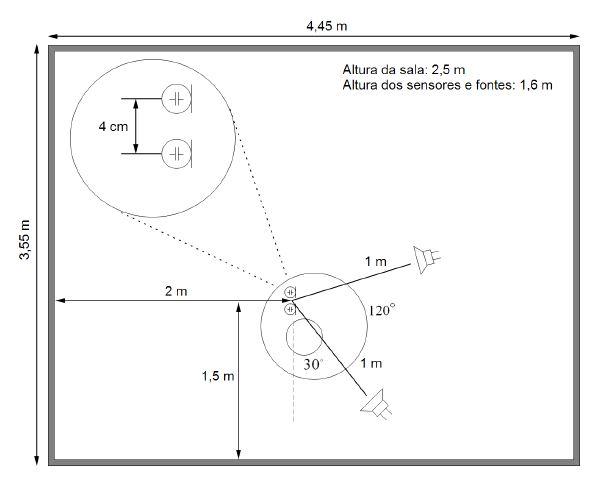
\includegraphics{environment.JPG}
    \caption{Configuração da sala utilizada nos testes. A sala possui as dimensões $4,45m \times 3,55m \times 2,5m$ (comprimento, largura e altura). Todo o ambiente é selado, i.e., não há portas ou janelas. Os microfones (sensores) encontram-se separados por uma distância de $4cm$ e o centro deste arranjo é representado pelo vetor $Mic_c$ = [2 1,5 1,6]$^T$. As fontes estão à distância de $1m$ do centro do arranjo de microfones e estão dispostas a $\frac{2\pi}{3}$ e $\frac{\pi}{6}$ em relação à ordenada.}
    \label{fig:environment}
\end{figure}


 \section{Análise dos Algoritmos}\label{sec:analysis}
    
    Nas condições de simulação descritas na Seção \ref{sec:simulation}, comparamos os métodos ICA-EBM e Natural ICA em relação aos resultados e à performance quanto à separação dos sinais. Vale ressaltar que o objetivo destes experimentos foi avaliar unicamente a etapa de separação dos sinais e, por isso, não houve qualquer alteração no método de resolução da permutação e de escalonamento. 
    
    Inicialmente, a simulalação foi feita com tempo de reverberação $T_{60}$ igual a 0.1s e comprimento da janela $L=2048$. Neste cenário, os sinais das fontes e dos sensores são mostrados nas Figuras \ref{fig:sources} e \ref{fig:sensors}, respectivamente. Após aplicar a STFT (definida na Seção \ref{sec:stft}) para transformar os sinais para o domínio da frequência e fazer a separação das fontes, incluindo tanto a etapa de pré-processamento (descrita na Seção \ref{sec:whitening}) quanto a de pós-processamento (apresentada na Seção \ref{sec:tdoa}), obtivemos as estimativas das fontes mostradas nas Figuras \ref{fig:icaebm} e \ref{fig:natica} para os métodos ICA-EBM e Natural ICA, respectivamente. Para este caso, ambos os métodos geraram boas estimativas das fontes, além de apresentarem desempenho similar.
    
    Posteriormente, aumentou-se o tempo de reverberação $T_{60}$ do ambiente de simulação, mantendo-se o comprimento da janela $L=2048$. Nas Figuras \ref{fig:icaebmsrc1} e \ref{fig:icaebmsrc2} (para o algoritmo ICA-EBM) e \ref{fig:naticasrc1} \ref{fig:naticasrc2} (para o algoritmo Natural ICA + FastICA), é mostrado como os indicadores de desempenho descritos na Seção \ref{metrics} evoluem com a variação deste parâmetro. As Figuras \ref{fig:icaebmconvergencets} e \ref{fig:naticaconvergencets} mostram o tempo de convergência para cada escolha do tempo de reverberação $T_{60}$ dos algoritmos ICA-EBM e Natural ICA + FastICA, respectivamente. Devido à queda no valor destas métricas com o aumento do tempo de reverberação $T_{60}$, é possível concluir que ambos os algoritmos passaram a ter suas estimativas degradadas. Além disso, apesar do desempenho ligeiramente superior do algoritmo ICA-EBM para todos os tempos de reverberação $T_{60}$, o algoritmo Natural ICA + FastICA apresenta um tempo de convergência significantemente menor para todos os tempos de reverberação $T_{60}$.
    
    Por fim, fixou-se o tempo de reverberação $T_{60}=0.5s$ e variou-se o tamanho da janela $L$ para os valores $256$, $512$, $1024$ e $2048$. O efeito deste parâmetro sobre as métricas de desempenho da Seção \ref{metrics} está representado nas Figuras \ref{fig:icaebmwindowsrc1} e \ref{fig:icaebmwindowsrc2} para o algoritmo ICA-EBM e \ref{fig:naticawindowsrc1} e \ref{fig:naticawindowsrc2} para o algoritmo Natural ICA + FastICA. As Figuras \ref{fig:icaebmconvergencewindow} e \ref{fig:naticaonvergencewindow} mostram o tempo de convergência dos algoritmos ICA-EBM e Natural ICA + FastICA, respectivamente, em função do comprimento da janela $L$. Podemos concluir que, dado este tempo de reverberação, a janela de comprimento $L=512$ apresenta melhor desempenho em ambos os métodos, mas o ICA-EBM leva consideravelmente menos tempo para convergir do que o Natural ICA + FastICA, mostrando-se mais adequado.
    
    \begin{figure}
        \centering
        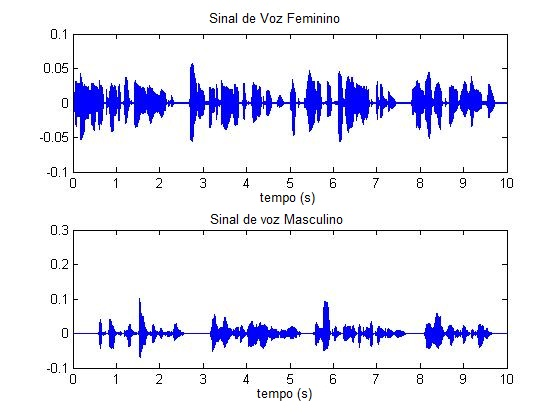
\includegraphics[scale=0.7]{sources.jpg}
            \caption{Sinais de cada uma das fontes no domínio do tempo.}
        \label{fig:sources}
        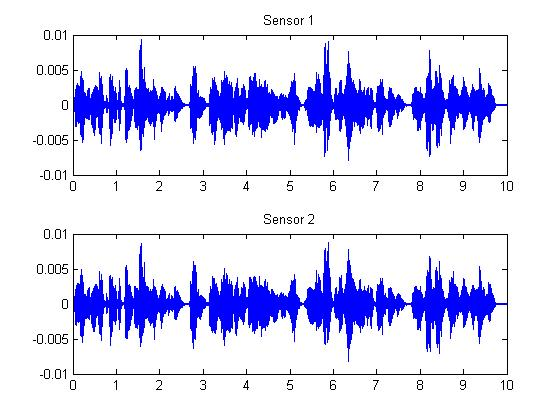
\includegraphics[scale=0.7]{sensors.jpg}
            \caption{Sinais em cada um dos sensores no domínio do tempo para $T_{60} = 0.1s$.}
        \label{fig:sensors}
    \end{figure}
    
    \begin{figure}
        \centering
        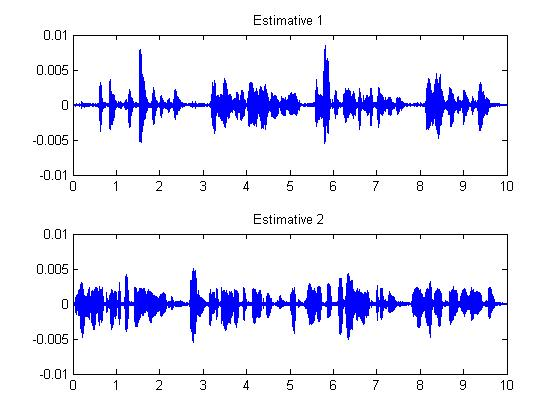
\includegraphics[scale=0.7]{estimatives_FASTICA.jpg}
        \caption{Sinais de estimativa das fontes obtidas pelo algoritmo ICA-EBM no domínio do tempo para $T_{60} = 0.1s$.}
        \label{fig:icaebm}
        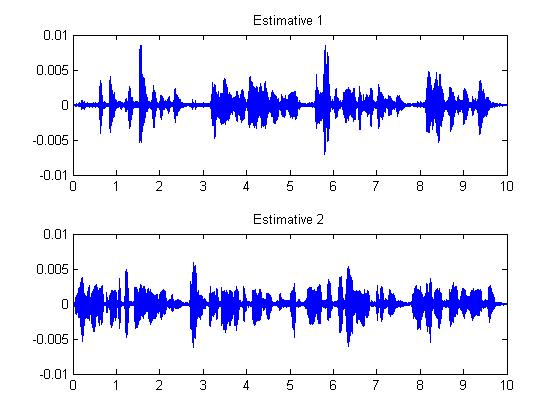
\includegraphics[scale=0.7]{estimatives_NATICA.jpg}
        \caption{Sinais de estimativa das fontes obtidas pelo algoritmo Natural ICA + FastICA  no domínio do tempo para $T_{60} = 0.1s$.}
        \label{fig:natica}
    \end{figure}
    
\begin{figure}
    \centering
    \subfigure[Métricas de desempenho para a estimativa da fonte 1.]
    {
        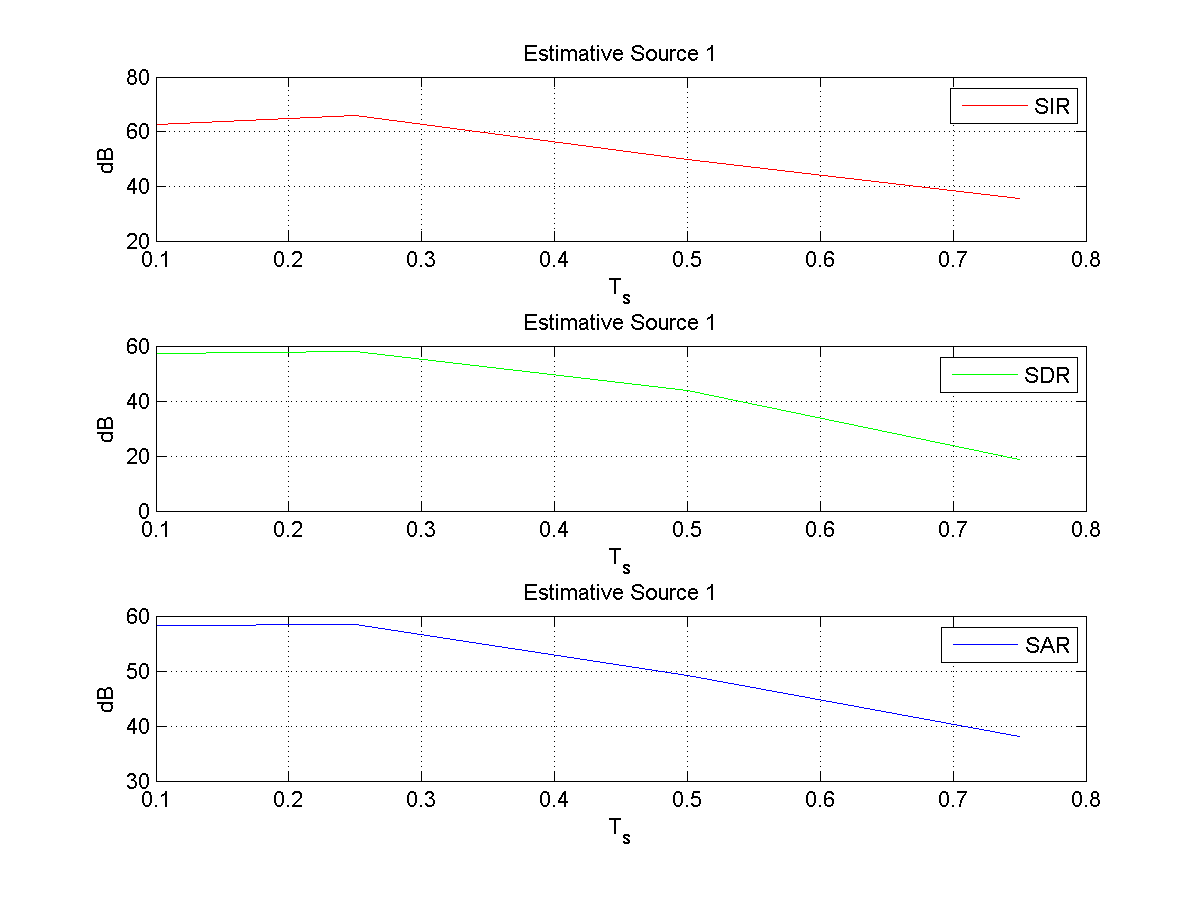
\includegraphics[scale=0.6]{figuras/reverb_estimative_1_fastica.png}
        \label{fig:icaebmsrc1}
    }
    \\
    \subfigure[Métricas de desempenho para a estimativa da fonte 2.]
    {
        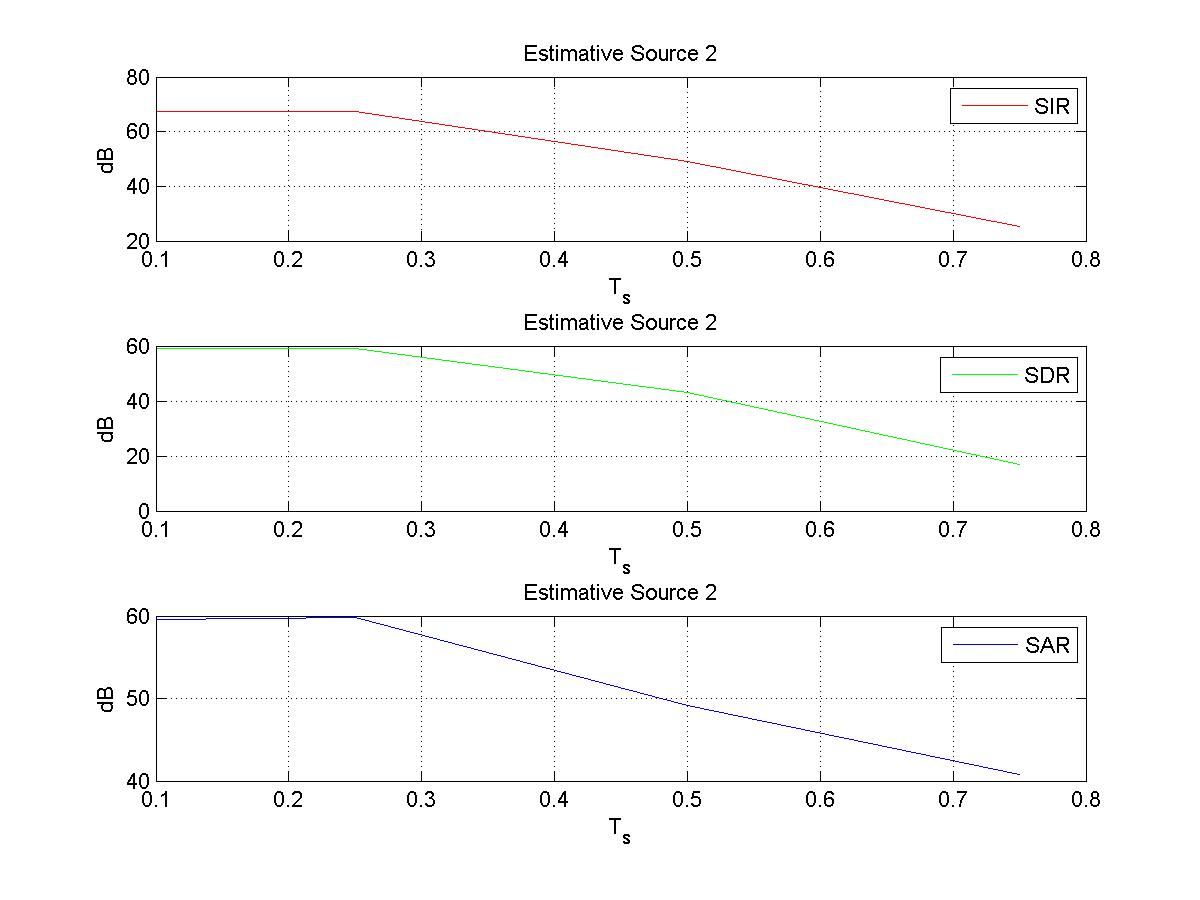
\includegraphics[scale=0.6]{figuras/reverb_estimative_2_fastica.png}
        \label{fig:icaebmsrc2}
    }
    \caption{Métricas de desempenho do algoritmo ICA-EBM em função do tempo de reverberação $T_{60}$. É possível verificar a queda do desempenho através da evolução dos valores das métricas SIR, SDR e SAR provocado pelo aumento do tempo de reverberação.}
    \label{fig:icaebmreverb}
\end{figure}

       
\begin{figure}
    \centering
    \subfigure[Métricas de desempenho para a estimativa da fonte 1.]
    {
        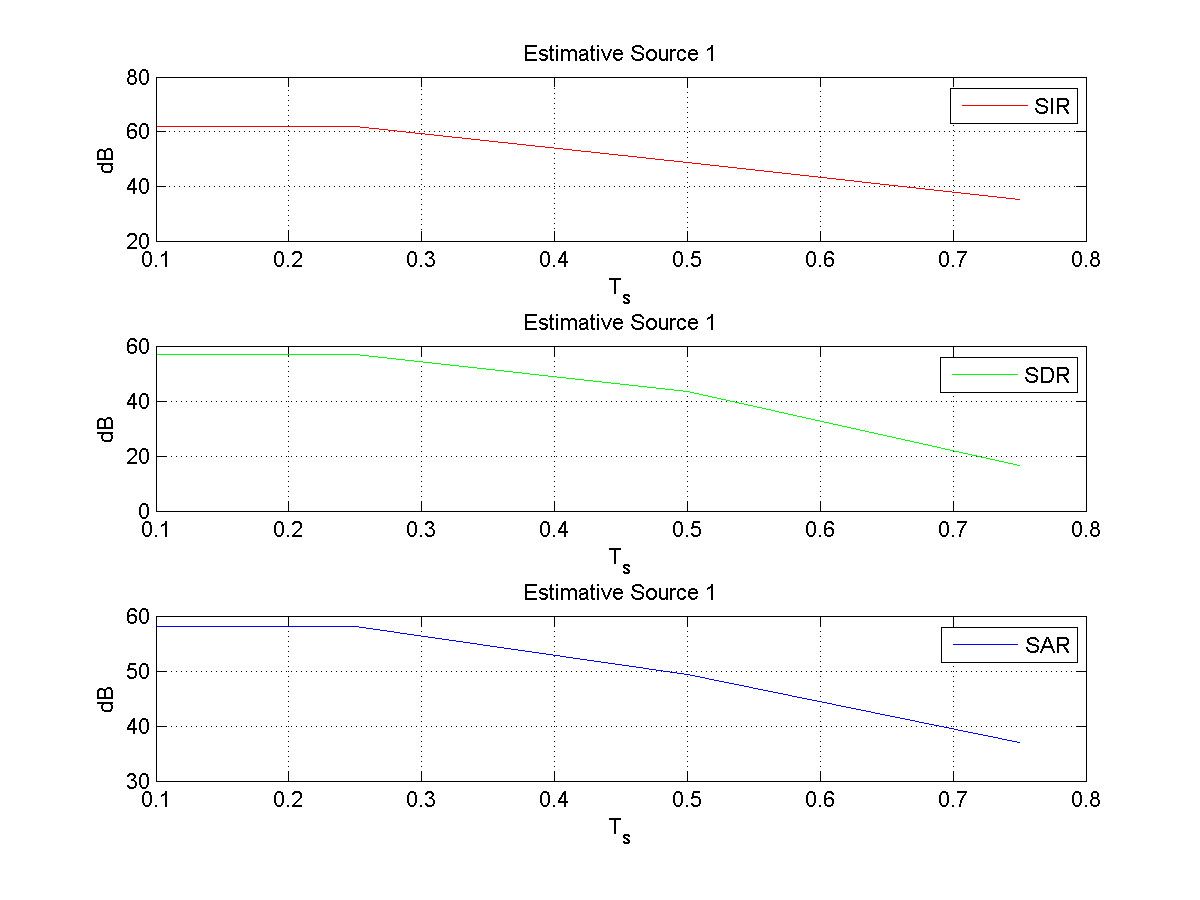
\includegraphics[scale=0.6]{figuras/reverb_estimative_1_natica.png}
        \label{fig:naticasrc1}
    }
    \\
    \subfigure[Métricas de desempenho para a estimativa da fonte 2.]
    {
        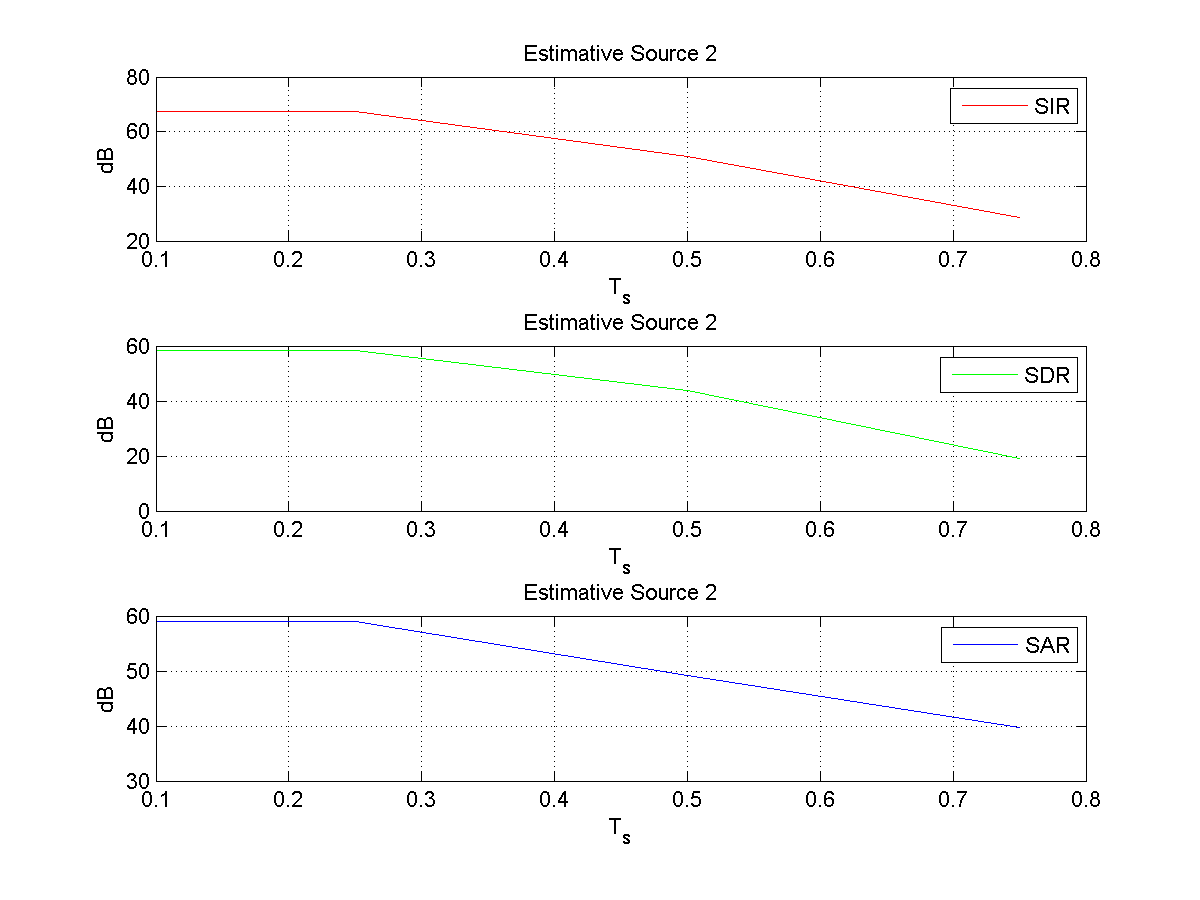
\includegraphics[scale=0.6]{figuras/reverb_estimative_2_natica.png}
        \label{fig:naticasrc2}
    }
    \caption{Métricas de desempenho do algoritmo Natural ICA + FastICA em função do tempo de reverberação $T_{60}$. É possível verificar a queda do desempenho através da evolução dos valores das métricas SIR, SDR e SAR provocado pelo aumento do tempo de reverberação.}
    \label{fig:naticareverb}
\end{figure}

       
\begin{figure}
    \centering
    \subfigure[Tempo de convergência para o algoritmo ICA-EBM.]
    {
        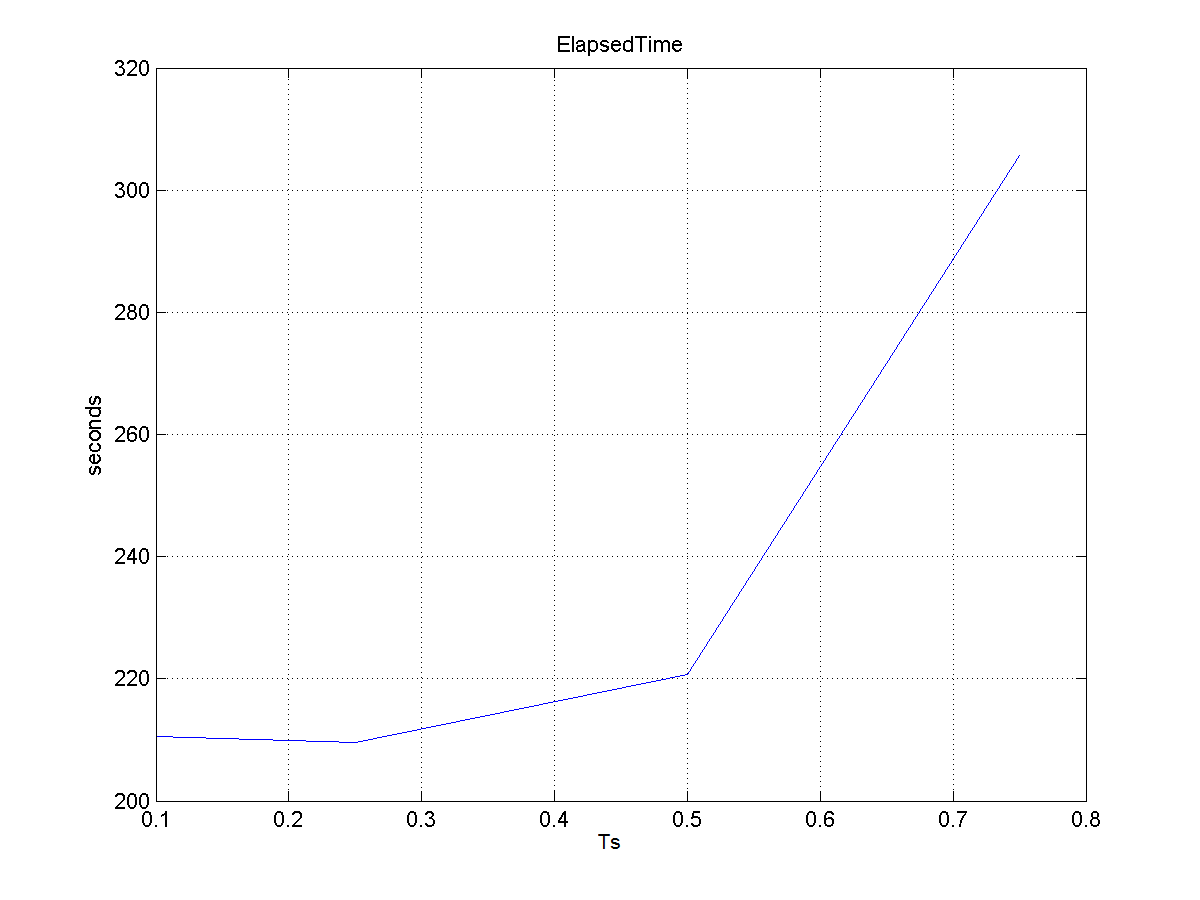
\includegraphics[scale=0.5]{figuras/convergence_ts_fastica.png}
        \label{fig:icaebmconvergencets}
    }
    \\
    \subfigure[Tempo de convergência para o algoritmo Natural ICA + FastICA.]
    {
        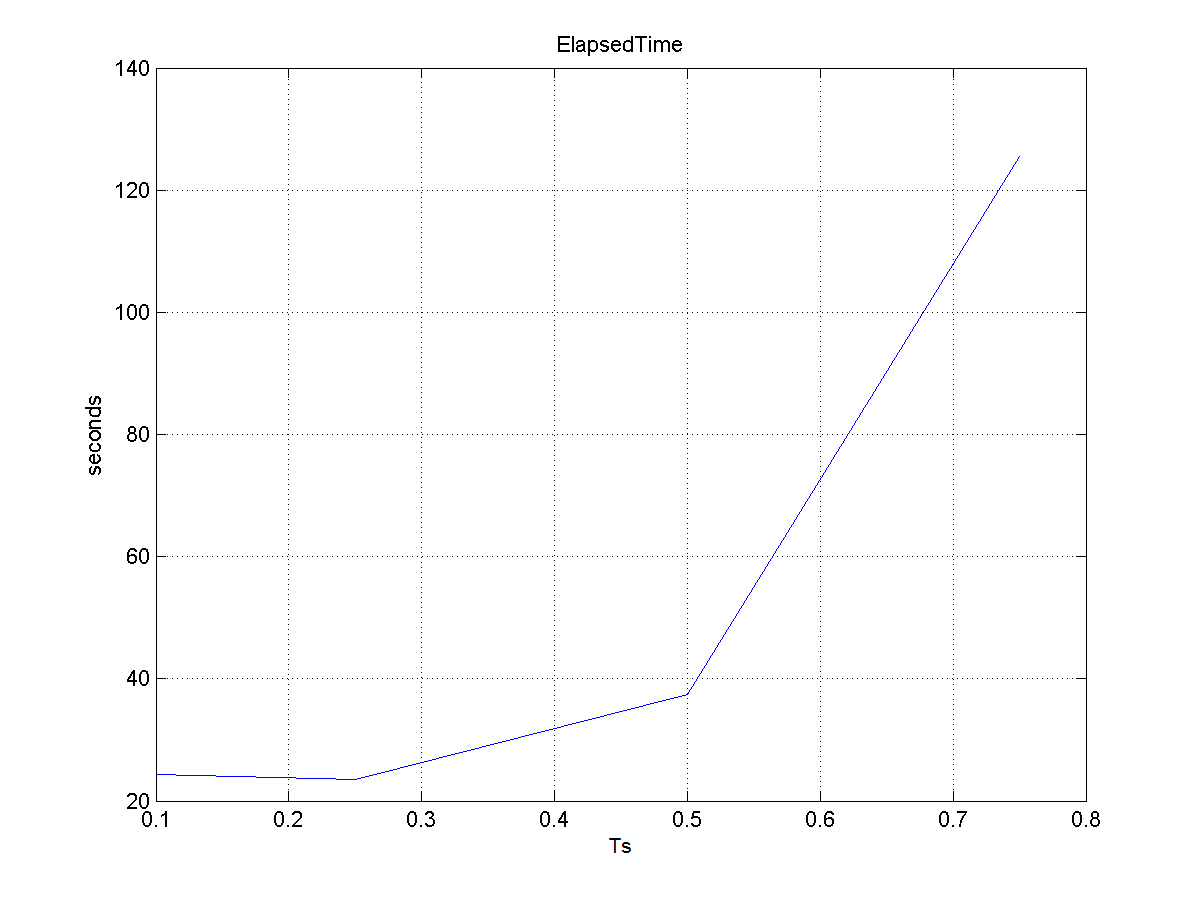
\includegraphics[scale=0.5]{figuras/convergence_ts_natica.png}
        \label{fig:naticaconvergencets}
    }
    \caption{Tempo de convergência dos algoritmos ICA-EBM e Natural ICA + FastICA em função do tempo de reverberação do ambiente $T_{60}$. É possível verificar que ambos os algoritmos levam mais tempo para convergir conforme o tempo de reverberação aumenta, mas o algoritmo Natural ICA + FastICA leva consideravelmente menos tempo do que o ICA-EBM para qualquer $T_{60}$.}
    \label{fig:naticareverb}
\end{figure}




 
\begin{figure}
    \centering
    \subfigure[Métricas de desempenho para a estimativa da fonte 1.]
    {
        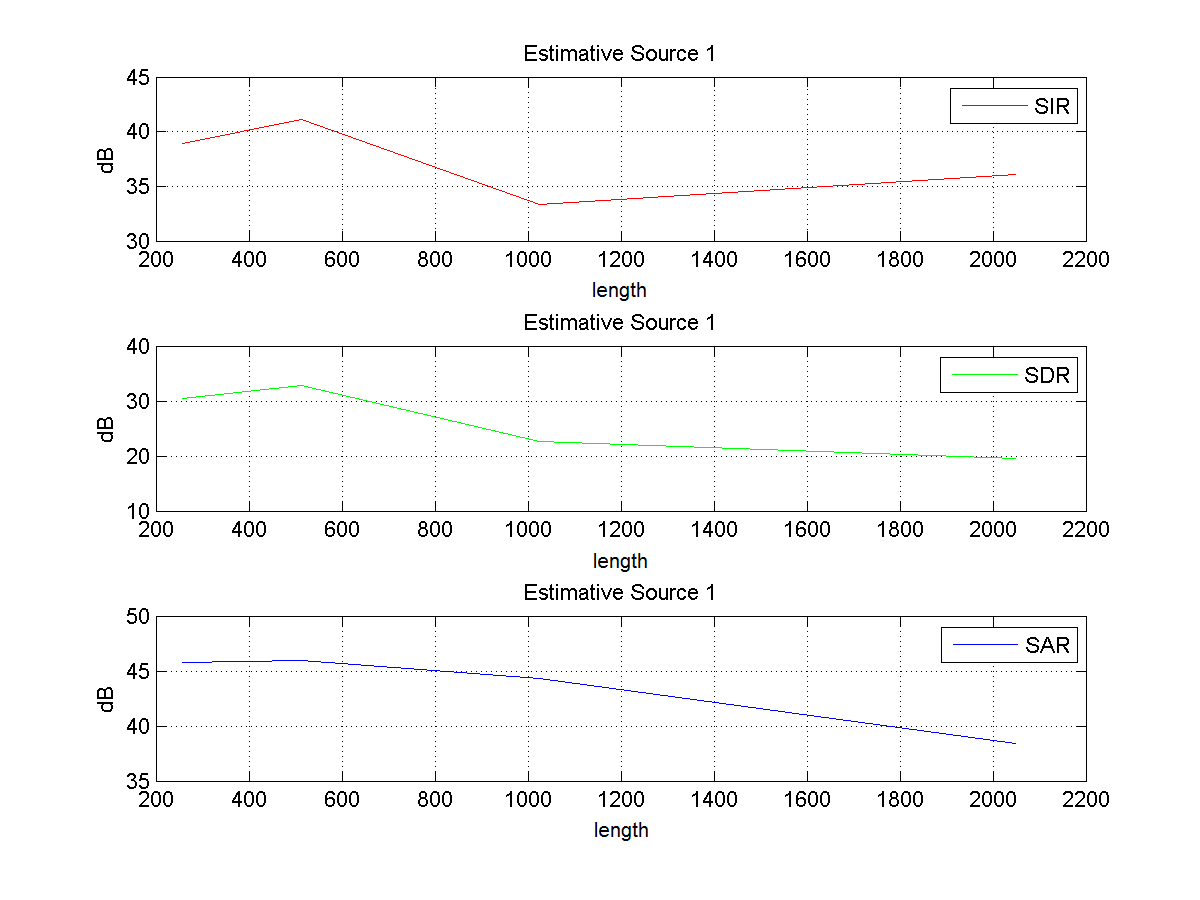
\includegraphics[scale=0.6]{figuras/window_estimative_1_Ts05_fastica.png}
        \label{fig:icaebmwindowsrc1}
    }
    \\
    \subfigure[Métricas de desempenho para a estimativa da fonte 2.]
    {
        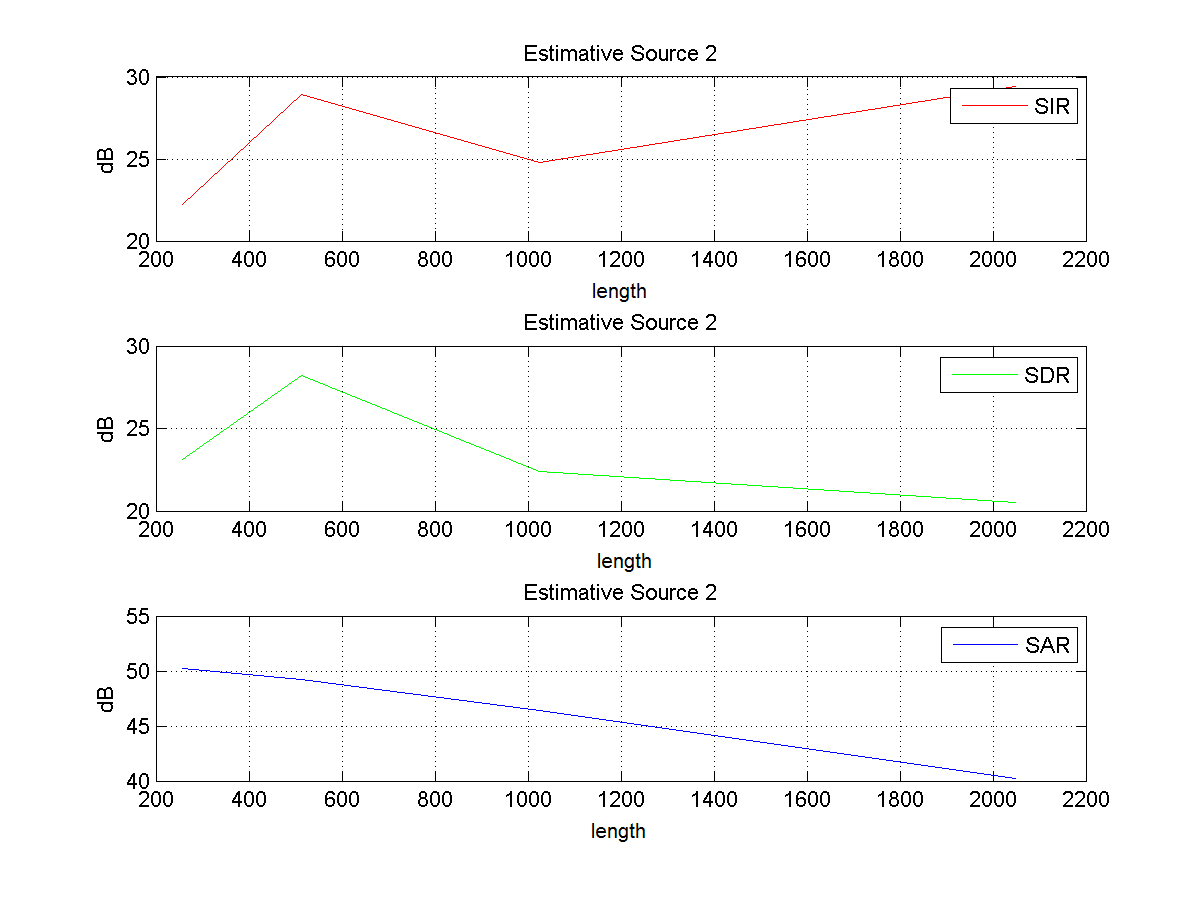
\includegraphics[scale=0.6]{figuras/window_estimative_2_Ts05_fastica.png}
        \label{fig:icaebmwindowsrc2}
    }
    \caption{Métricas de desempenho do algoritmo ICA-EBM em função do comprimento da janela $L$. A janela de comprimento $L=512$ possui um desempenho superior.}
    \label{fig:icaebmwindow}
\end{figure}

       
\begin{figure}
    \centering
    \subfigure[Métricas de desempenho para a estimativa da fonte 1.]
    {
        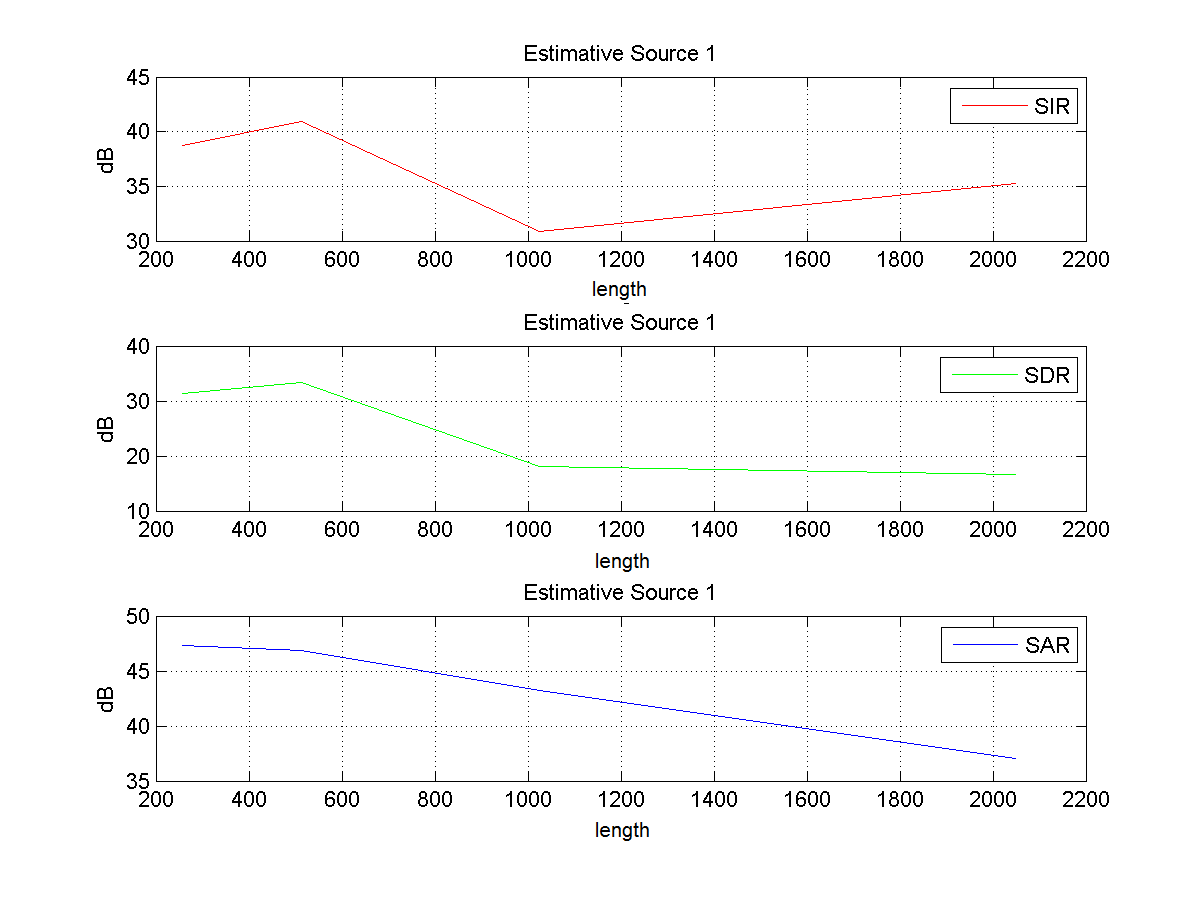
\includegraphics[scale=0.6]{figuras/window_estimative_1_Ts05_natica.png}
        \label{fig:naticawindowsrc1}
    }
    \\
    \subfigure[Métricas de desempenho para a estimativa da fonte 2.]
    {
        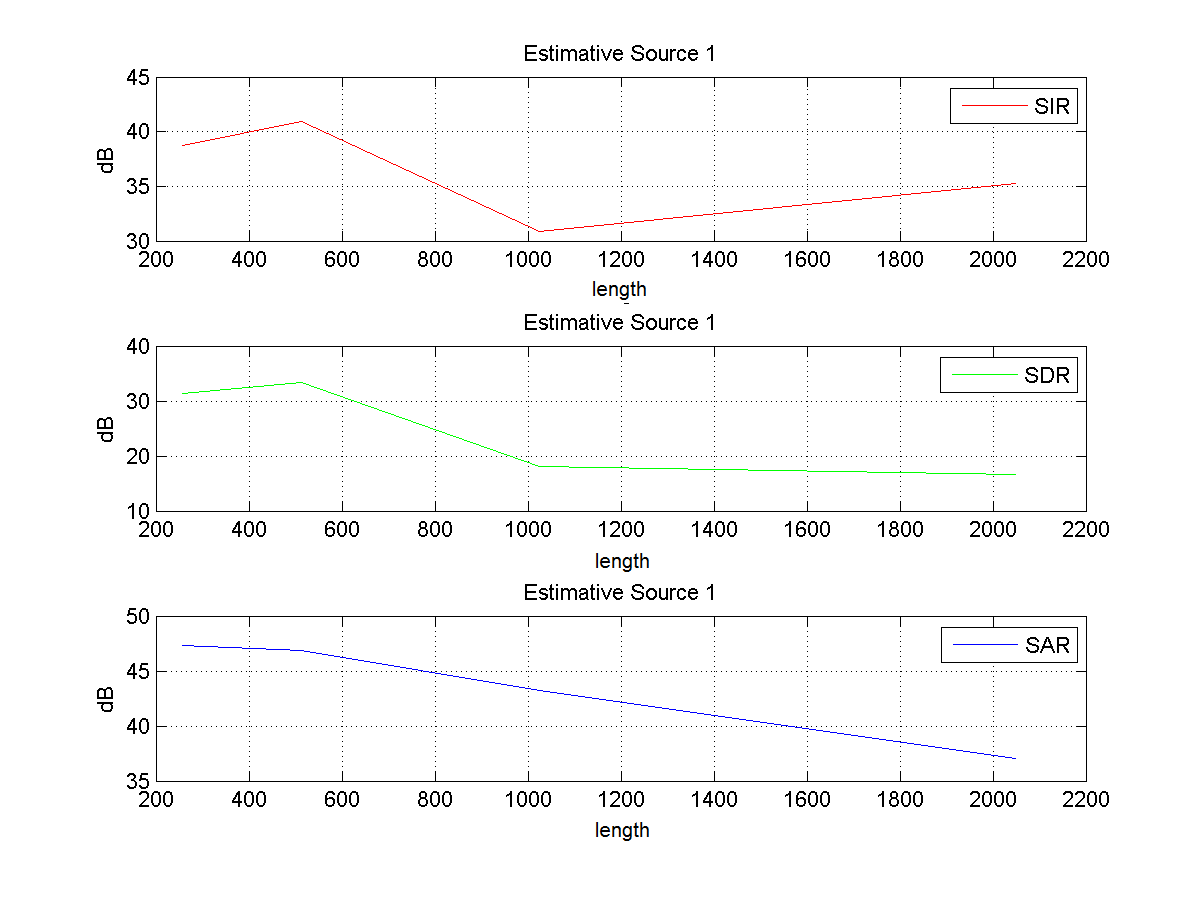
\includegraphics[scale=0.6]{figuras/window_estimative_1_Ts05_natica.png}
        \label{fig:naticawindowsrc2}
    }
    \caption{Métricas de desempenho do algoritmo ICA-EBM e Natural ICA + FastICA em função do comprimento da janela $L$. A janela de comprimento $L=512$ possui um desempenho superior.}
    \label{fig:naticawindow}
\end{figure}


\begin{figure}
    \centering
    \subfigure[Tempo de convergência para o algoritmo ICA-EBM.]
    {
        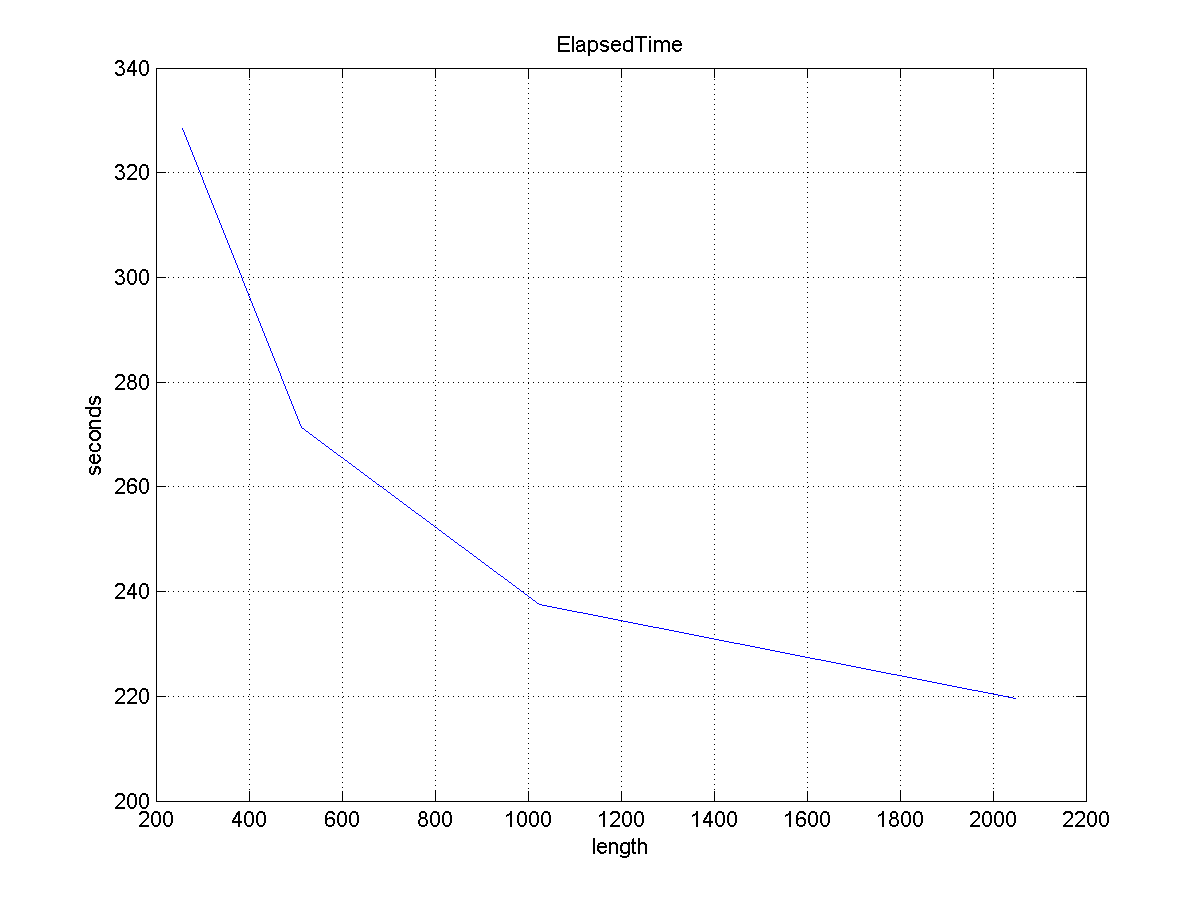
\includegraphics[scale=0.5]{figuras/convergence_fastica.png}
        \label{fig:icaebmconvergencewindow}
    }
    \\
    \subfigure[Tempo de convergência para o algoritmo Natural ICA + FastICA.]
    {
        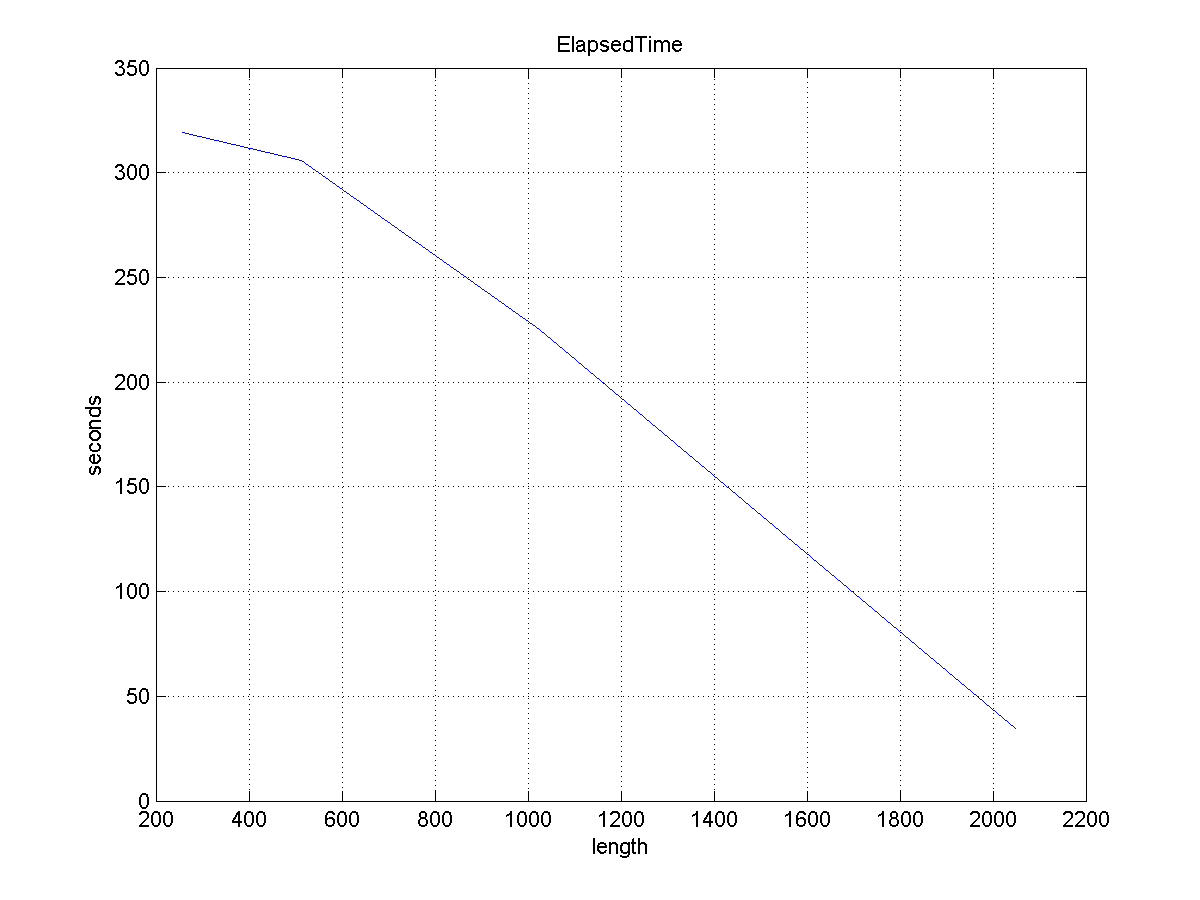
\includegraphics[scale=0.5]{figuras/convergence_natica.png}
        \label{fig:naticaonvergencewindow}
    }
    \caption{Tempo de convergência dos algoritmos ICA-EBM e Natural ICA + FastICA em função do comprimento da janela $L$. O algoritmo ICA-EBM possui um tempo de convergência mais baixo até a janela de $L=1024$. Após este ponto, o algoritmo Natural ICA + FastICA passa a ter uma queda bem mais acentuada no seu tempo de convergência em relação ao ICA-EBM. Se considerarmos a janela de comprimento $L=512$ como sendo a melhor escolha, o algoritmo ICA-EBM se mostra mais vantajoso. }
    \label{fig:naticawindowconvergence}
\end{figure}




% ---------------------------------------------------------------
% Bibliografia
% ---------------------------------------------------------------
\normalsize
\cleardoublepage
\addcontentsline{toc}{chapter}{Referências Bibliográficas}
\bibliographystyle{coppe}
\bibliography{biblio}

% ---------------------------------------------------------------
% Apêndices 
% ---------------------------------------------------------------
   \appendix
   % ---------------------------------------------------------------
   % Apêndice A - Teste
   % ---------------------------------------------------------------
   \chapter{Ambiente de Teste}
   \label{ApendiceA}
   \label{app:A}

Simulamos a resposta de frequência de uma sala utilizando o algoritmo Image-Source Model \cite{simulation}.

sala utilizada nas simulações tem dimensões 4,45m × 3, 55m × 2,5m (largura × comprimento × altura). A sala é completamente selada, para fins de simulação. Além disso, o coeficiente de absorção de todos os lados é o mesmo, como se todos fossem feitos do mesmo material. O material utilizado varia com o tempo de reverberação, e o algoritmo de simulação calcula o coeficiente de absorção de cada lado da sala dependendo do
tempo de reverberação escolhido. O arranjo de microfones é linear e foi montado em torno do ponto $\mathpzc{Mic_c = [2 1,5 1,6]^T}$. São 2 microfones e fontes. As fontes foram distribuídas em torno do centro do arranjo, com dois parâmetros para identificá-las: o DOA de cada uma, e a distância delas até o arranjo. O parâmetro mais importante da sala é o tempo de reverberação. O tempo utilizado nesta dissertação é o $\mathpzc{T_60}$, que é o tempo requerido para que as reflexões cheguem a 60 dB abaixo do nível do som direto.

As fontes utilizadas foram do SASSEC e são trechos de sinal de voz de 10 segundos de duração cada, amostrados a 16 kHz. Decimamos os sinais para que a frequência de amostragem caísse para 8 kHz. As projeções do ambiente estão representados na Figura \ref{fig:environment}

\begin{figure}
    \centering
    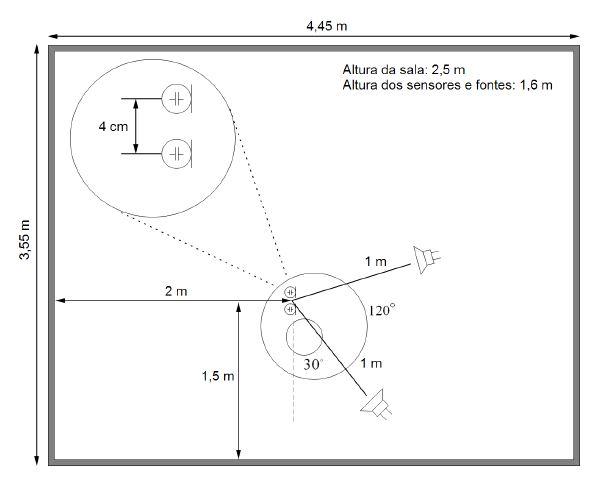
\includegraphics{environment.JPG}
    \caption{Configuração da sala utilizada nos testes.}
    \label{fig:environment}
\end{figure}

\backmatter

\end{document}
